\documentclass[a4paper, 14pt]{extarticle}

\usepackage{../latexDependencies/misc/preamble2}

\geometry{a4paper}

% Название дисциплины
\newcommand{\subject}{Численные методы} 

% Тип работы
% lab - для лабораторной работы 
% hw  - для домашней     работы
\newcommand{\task}{hw} 

% Номер работы
\newcommand{\taskNumber}{2-2} 

% Название работы
\newcommand{\taskNameOne}{Определение списка полиномов интерполяционного} 
\newcommand{\taskNameTwo}{сплайна третьей степени единичного дефекта} 
\newcommand{\taskNameThree}{для заданной сеточной функции} 

% Имя студента
\newcommand{\studentName}{Очкин Н.В.}

% Имя преподававателя
\newcommand{\teacherName}{Кутыркин В.А.}

% Группа
\newcommand{\group}{ФН11-52Б}

% Вариант
\newcommand{\variant}{9}

\begin{document}

\graphicspath{ {../latexDependencies/images} } 
\normalsize

\newcommand{\printTask}{%
    \ifthenelse{\equal{\task}{lab}}{%
        лабораторной%
    }{%
        \ifthenelse{\equal{\task}{hw}}{%
            домашней%
        }{%
            Неизвестный тип задания%
        }%
    }%
}

\begin{titlepage}

    \begin{center}
        {\footnotesize \itshape Федеральное государственное бюджетное 
                       образовательное учреждение высшего образования}
    \end{center}

    \begin{minipage}[c]{0.1\textwidth}
        
\includegraphics[width=1.1\textwidth]{iconBMSTU}
    \end{minipage}
    \hfill
    \begin{minipage}[c]{0.9\textwidth}
        \centering
        \itshape
        \bfseries
        \small
        \guillemotleft Московский государственный технический университет \\
        имени Н.Э. Баумана\guillemotright \\
        (национальный исследовательский университет) \\
        (МГТУ им. Н.Э. Баумана) 
    \end{minipage}

    \vspace{0.5cm}
    \noindent\rule{\textwidth}{2pt} \\

    \noindent\uline{\textbf{ФАКУЛЬТЕТ} ФУНДАМЕНТАЛЬНЫЕ НАУКИ} \\
    \vspace{-5pt} \\
    \noindent\uline{\textbf{КАФЕДРА} ВЫЧИСЛИТЕЛЬНАЯ МАТЕМАТИКА И МАТЕМАТИЧЕСКАЯ} \\
    \vspace{-5pt} \\
    \noindent\uline{ФИЗИКА (ФН11)} \\
    \vspace{-5pt} \\
    \noindent\uline{\textbf{НАПРАВЛЕНИЕ ПОДГОТОВКИ} МАТЕМАТИКА И КОМПЬЮТЕРНЫЕ} \\
    \vspace{-5pt} \\
    \noindent\uline{НАУКИ (02.03.01)} \\

    \begin{center}
        \bfseries
        \textsc{О т ч е т} \\[10pt]
        по \printTask {} работе \textnumero {} \taskNumber
    \end{center}

    \vspace{10pt}

    \hspace{10pt} 
    \noindent \textbf{Название \printTask {} работы:} \par
    \vspace{5pt}
    \hspace{10pt} 
    \noindent \textbf{\uline{\taskNameOne}} \vspace{5pt} \\
    \null\hspace{31pt} 
    \textbf{\uline{\taskNameTwo}} \vspace{5pt} \\
    \null\hspace{31pt} 
    \textbf{\uline{\taskNameThree}}

    \vspace{10pt}

    \begin{center}
        \bfseries
        Вариант \textnumero {} \variant
    \end{center}

    \vspace{20pt}

    \hspace{10pt} 
    \noindent \textbf{Дисциплина:} \par
    \vspace{10pt}
    \hspace{10pt} 
    \noindent {\large \subject}

    \vspace{10pt}

    \begin{flushright}
        \renewcommand{\arraystretch}{3}
        \begin{tabular}{r r r}
            \multicolumn{1}{l}{Студент группы \uline{\group}} & 
            $\quad \underset{\text{(Подпись, дата)}}{\underline{\hspace{3cm}}} \quad$ & 
            \multicolumn{1}{c}{$\underset{\text{(И.О. Фамилия)}}{\uline{\textbf{\studentName}}}$} \\

            \multicolumn{1}{l}{Преподаватель} & 
            $\quad \underset{\text{(Подпись, дата)}}{\underline{\hspace{3cm}}} \quad$ & 
            \multicolumn{1}{c}{$\underset{\text{(И.О. Фамилия)}}{\uline{\textbf{\teacherName}}}$} \\
        \end{tabular}
    \end{flushright}

    \vfill

    \begin{center}
        \small
        Москва, 2024
    \end{center}
\end{titlepage}


\newgeometry{left=25mm, right=25mm, top=20mm, bottom=20mm}

\graphicspath{ {../latexDependencies/images/HW2-2} }

% Customize section, subsection, subsubsection and paragraph styles
\titleformat{\section}
  {\normalfont\large\bfseries}{\thesection}{1em}{}

\titleformat{\subsection}
  {\normalfont\normalsize\bfseries}{\thesubsection}{1em}{}

\titleformat{\subsubsection}
  {\normalfont\small\bfseries}{\thesubsubsection}{1em}{}

\titleformat{\paragraph}
  {\small\small\bfseries}{\theparagraph}{1em}{}

% \thispagestyle{empty}

% \null\newpage

% \setcounter{tocdepth}{5}
% \setcounter{secnumdepth}{5}

% \pagenumbering{roman}

% \tableofcontents
% \newpage

% \pagenumbering{arabic}
% \setcounter{page}{1}

\setstretch{1}
\linespread{1.1}

\setlength{\parindent}{0pt}

\fontsize{12pt}{16pt}\selectfont

% \definecolor{myblue}{HTML}{0A88C2}
% \definecolor{myred}{HTML}{FF1B1C}
% \definecolor{mygreen}{HTML}{386641}

% \lstdefinestyle{mystyle}{
%     basicstyle=\ttfamily\footnotesize,
%     keywordstyle=\color{myblue},
%     stringstyle=\color{myred},
%     commentstyle=\color{green!50!black},
%     showstringspaces=false,
%     frame=leftline, 
%     framesep=10pt, 
% }

% % Set the style for Python code
% \lstset{style=mystyle, extendedchars=\true}

% --------------------------------------START--------------------------------------

\section*{Задание}\vspace{-20pt}\rule{\linewidth}{0.1mm}

На отрезке [0; 2] задана равномерная сетка $A = \langle \tau_0, \tau_1, \dots, \tau_k \rangle$, 
где k=20, с шагом $h = 0.1 = \text{stp}(A)$ и определена функция 
\begin{equation*}
    f(\tau) = 2 (54 - n) \sin(\pi \tau) \sqrt{1 + 2 N (\tau - 0.5)^2 + N^2},
\end{equation*}
где $n$ – номер группы и $N$ – номер студента в журнале группы. Для $A$ -сеточной функции
$\upgt y = \hat{A} (f) = \left[ y_0, y_1, \dots, y_k \right\rangle \in \upgt \mathbb{R}^{|A|}(A)$,
где $y_i = f(\tau_i)$ для $i = \overline{0, k}$, решить задачу $A$ -
интерполяции сеточной функции $\upgt y$ с помощью сплайна $\text{spl}_3(A; \upgt y)$
3-ей степени дефекта 1. Затем сравнить в узлах равномерной сетки 
$B = \langle \theta_0, \theta_1, \dots, \theta_{2k} \rangle$ $(\text{stp}(B)=0.05)$ 
отрезка [0;2] значения функции $f(\tau)$ и сплайна $\text{spl}_3(A; \upgt y)$ и, 
кроме того, значения их производных, т.е. значения функций. Результаты 
проиллюстрировать графически.

\section*{Исходные данные}\vspace{-20pt}\rule{\linewidth}{0.1mm}

\begin{equation*}
    [0; 2] \qquad k=20 \qquad h=0.1 \qquad N = 0 \qquad n=52
\end{equation*}

\begin{equation*}
    f(\tau) = 2 (54 - n) \sin(\pi \tau) \sqrt{1 + 2 N (\tau - 0.5)^2 + N^2}
\end{equation*}

\section*{{Ход выполнения работы}}\vspace{-20pt}\rule{\linewidth}{0.1mm}

Для построения равнмоерной сетки с 21-м узлом воспользуемся следующей формулой:
\begin{equation*}
  x_i = a + i \cdot h \qquad i=0,1,2,...,k,
\end{equation*}
где $h = \frac{b - a}{k}$.\\

Также вычислим значения функции $f(\tau)$ в узлах:
\begin{equation*}
  y_i = f(x_i) \qquad i=0,1,2,...,k
\end{equation*}

Итого получим следующие точки:

\begin{multicols}{3}
    \begin{enumerate}[itemsep=5pt]
        \item (x: 0.0, y: 0.0)
        \item (x: 0.1, y: 11.388)
        \item (x: 0.2, y: 21.5)
        \item (x: 0.3, y: 29.432)
        \item (x: 0.4, y: 34.487)
        \item (x: 0.5, y: 36.222)
        \item (x: 0.6, y: 34.487)
        \item (x: 0.7, y: 29.432)
        \item (x: 0.8, y: 21.5)
        \item (x: 0.9, y: 11.388)
        \item (x: 1.0, y: 0.0)
        \item (x: 1.1, y: -11.627)
        \item (x: 1.2, y: -22.406)
        \item (x: 1.3, y: -31.295)
        \item (x: 1.4, y: -37.386)
        \item (x: 1.5, y: -40.0)
        \item (x: 1.6, y: -38.755)
        \item (x: 1.7, y: -33.618)
        \item (x: 1.8, y: -24.929)
        \item (x: 1.9, y: -13.386)
        \item (x: 2.0, y: -0.0)
    \end{enumerate} 
\end{multicols}

Построим график по полученным точкам:

\begin{center}
    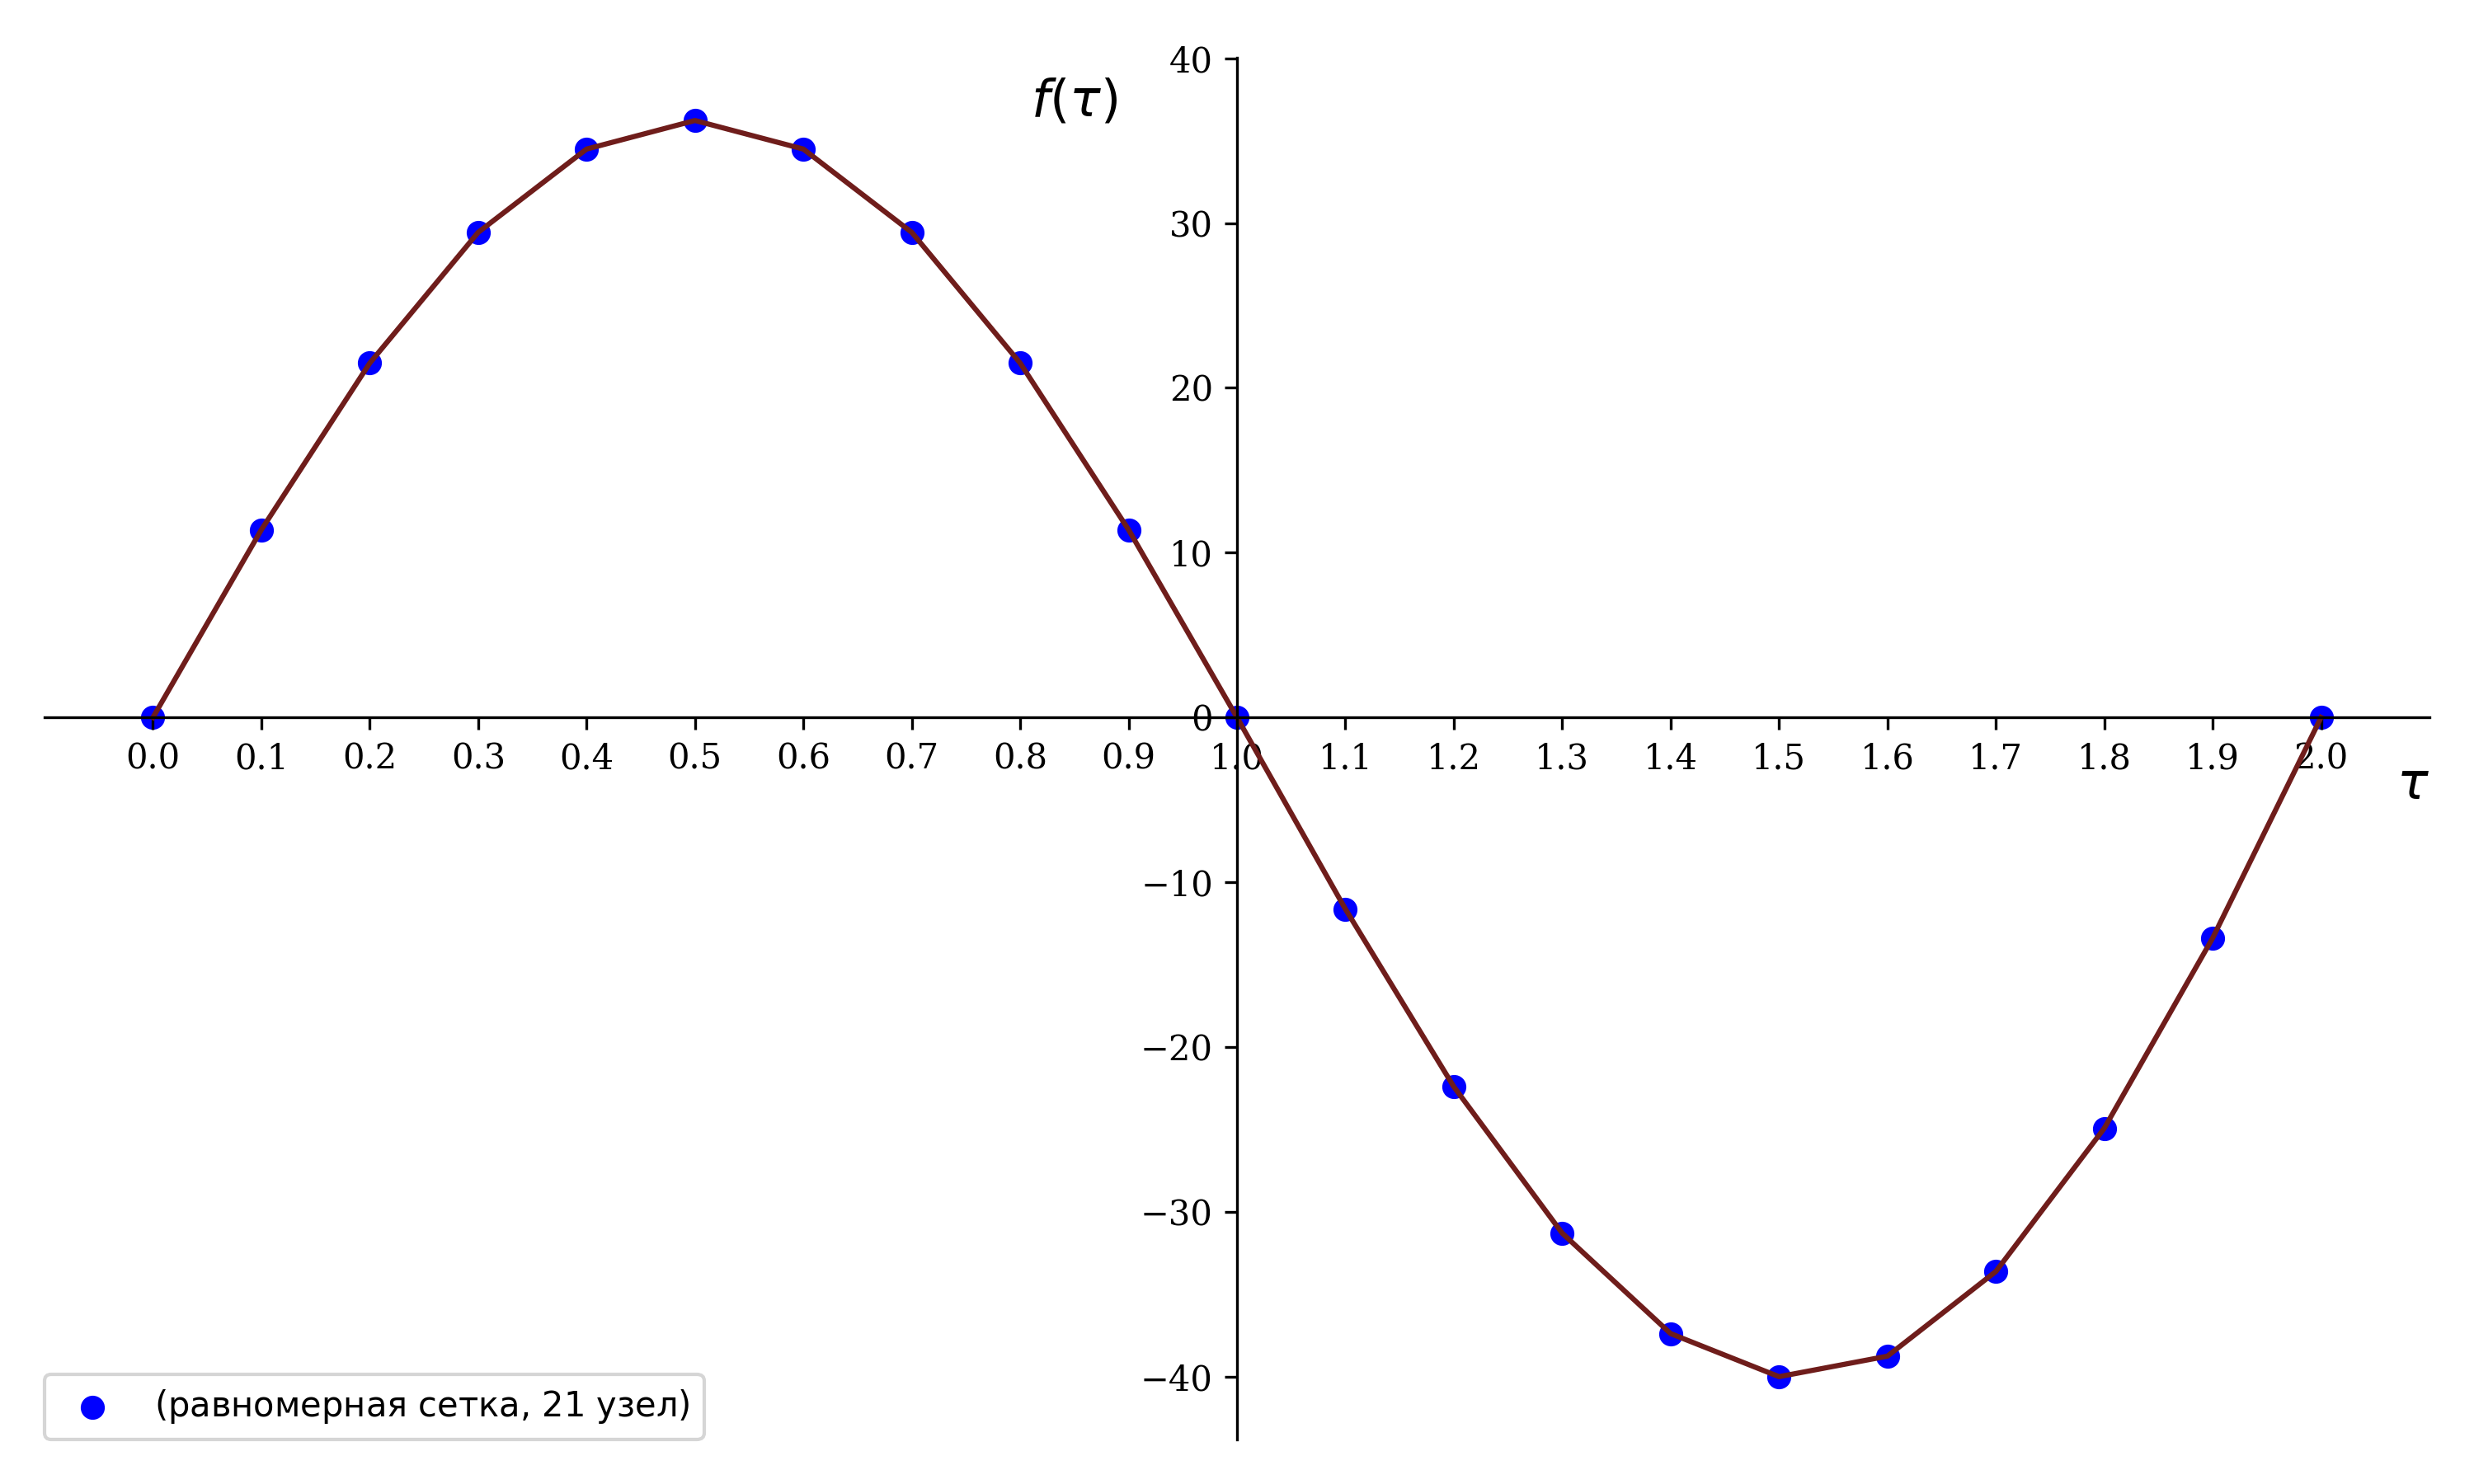
\includegraphics[width=1\textwidth]{main_func_20}
\end{center}

Теперь найдем коэффициенты сплайна:

\begin{equation}
    S_i(t) = a_i + b_i (t - \tau_{i-1}) + c_i (t - \tau_{i-1})^2 + d_i (t - \tau_{i-1})^3  
\end{equation}

\vspace{10pt}

\begin{equation}
    h_i = \tau_i - \tau_{i - 1} \qquad i \in \langle 1, 2, \dots, k \rangle 
\end{equation}
\begin{equation*}
    h = \langle 0.1, 0.1, 0.1, 0.1, 0.1, 0.1, 0.1, 0.1, 0.1, 0.1, 0.1, 0.1, 0.1, 0.1, 0.1, 0.1, 0.1, 0.1, 0.1, 0.1 \rangle 
\end{equation*}

\vspace{10pt}

\begin{equation}
    a_i = y_{i-1} \qquad i \in \langle 1, \dots, k \rangle 
\end{equation}
\begin{equation*}
    a = \langle 0.0, 11.38794, 21.49977, 29.43221, \dots, -24.92875, -13.38611 \rangle 
\end{equation*}

\vspace{10pt}

\begin{equation}
    g_i = \cfrac{a_{i+1} - a_i}{h_i} \qquad i \in \langle 1, \dots, k-1 \rangle  
\end{equation}
\begin{equation*}
    g = \langle 113.87937, 101.11831, 79.32444, 50.54309, \dots, 86.88999, 115.4264 \rangle 
\end{equation*}

\vspace{10pt}

\begin{equation}
    \begin{cases}
        c_1 = 0 \\
        h_i c_i + 2 (h_i + h_{i+1}) c_{i+1} + h_{i+1} c_{i+2} = 3 (g_{i+1} - g_i) \qquad i \in \langle 1, \dots, k-2 \rangle \\
        c_k = 0
    \end{cases}
\end{equation}

% \newpage

Представим (5) в матричном виде

\begin{equation*}
    \begin{pmatrix}
        2(h_1 + h_2) & h_2 & 0 & \cdots & 0 \\
        h_2 & 2(h_2 + h_3) & h_3 & \cdots & 0 \\
        0 & h_3 & 2(h_3 + h_4) & \cdots & 0 \\
        \vdots & \vdots & \vdots & \ddots & \vdots \\
        0 & 0 & 0 & \cdots & 2(h_{k-2} + h_{k-1})
        \end{pmatrix}
        \begin{pmatrix}
        c_2 \\
        c_3 \\
        \vdots \\
        c_{k-1}
        \end{pmatrix}
        = 3
        \begin{pmatrix}
        g_2 - g_1 \\
        g_3 - g_2 \\
        \vdots \\
        g_{k-1} - g_{k-2}
    \end{pmatrix}
\end{equation*}

Откуда находим значения $c_1, c_2, \dots, c_k$:

\begin{equation*}
    c = \langle 0, -68.25541, -109.81016, -146.31981, -168.35114, \dots, 170.54982, 0 \rangle 
\end{equation*}

Теперь мы можем найти два последних коэффициента:

\begin{gather}
    b_i = g_i - \cfrac{h_i}{3} (2 c_i + c_{i+1}) \qquad i \in \langle 1, \dots, k-1 \rangle \\
    b_k = b_{k-1} + h_{k-1} (c_{k-1} + c_k) 
\end{gather}
\begin{equation*}
    b = \langle 116.15455, 109.32901, 91.52245, 65.90945, \dots, 104.05641, 121.11139 \rangle 
\end{equation*}

% \vspace{10pt}

\begin{gather}
    d_i = \cfrac{1}{3 h_i} (c_{i+1} - c_i) \qquad i \in \langle 1, \dots, k-1 \rangle \\
    d_k = \cfrac{1}{h_k^3} (y_k - a_k - b_k h_k - c_k h_k^2) 
\end{gather}
\begin{equation*}
    d = \langle -227.51803, -138.51583, -121.69885, -73.43777, \dots, -568.49939, 1274.96921 \rangle 
\end{equation*}

Подставляя (2)-(9) в (1) получим искомый сплайн. Построим его график на ранее 
найденных узлах:

\begin{center}
    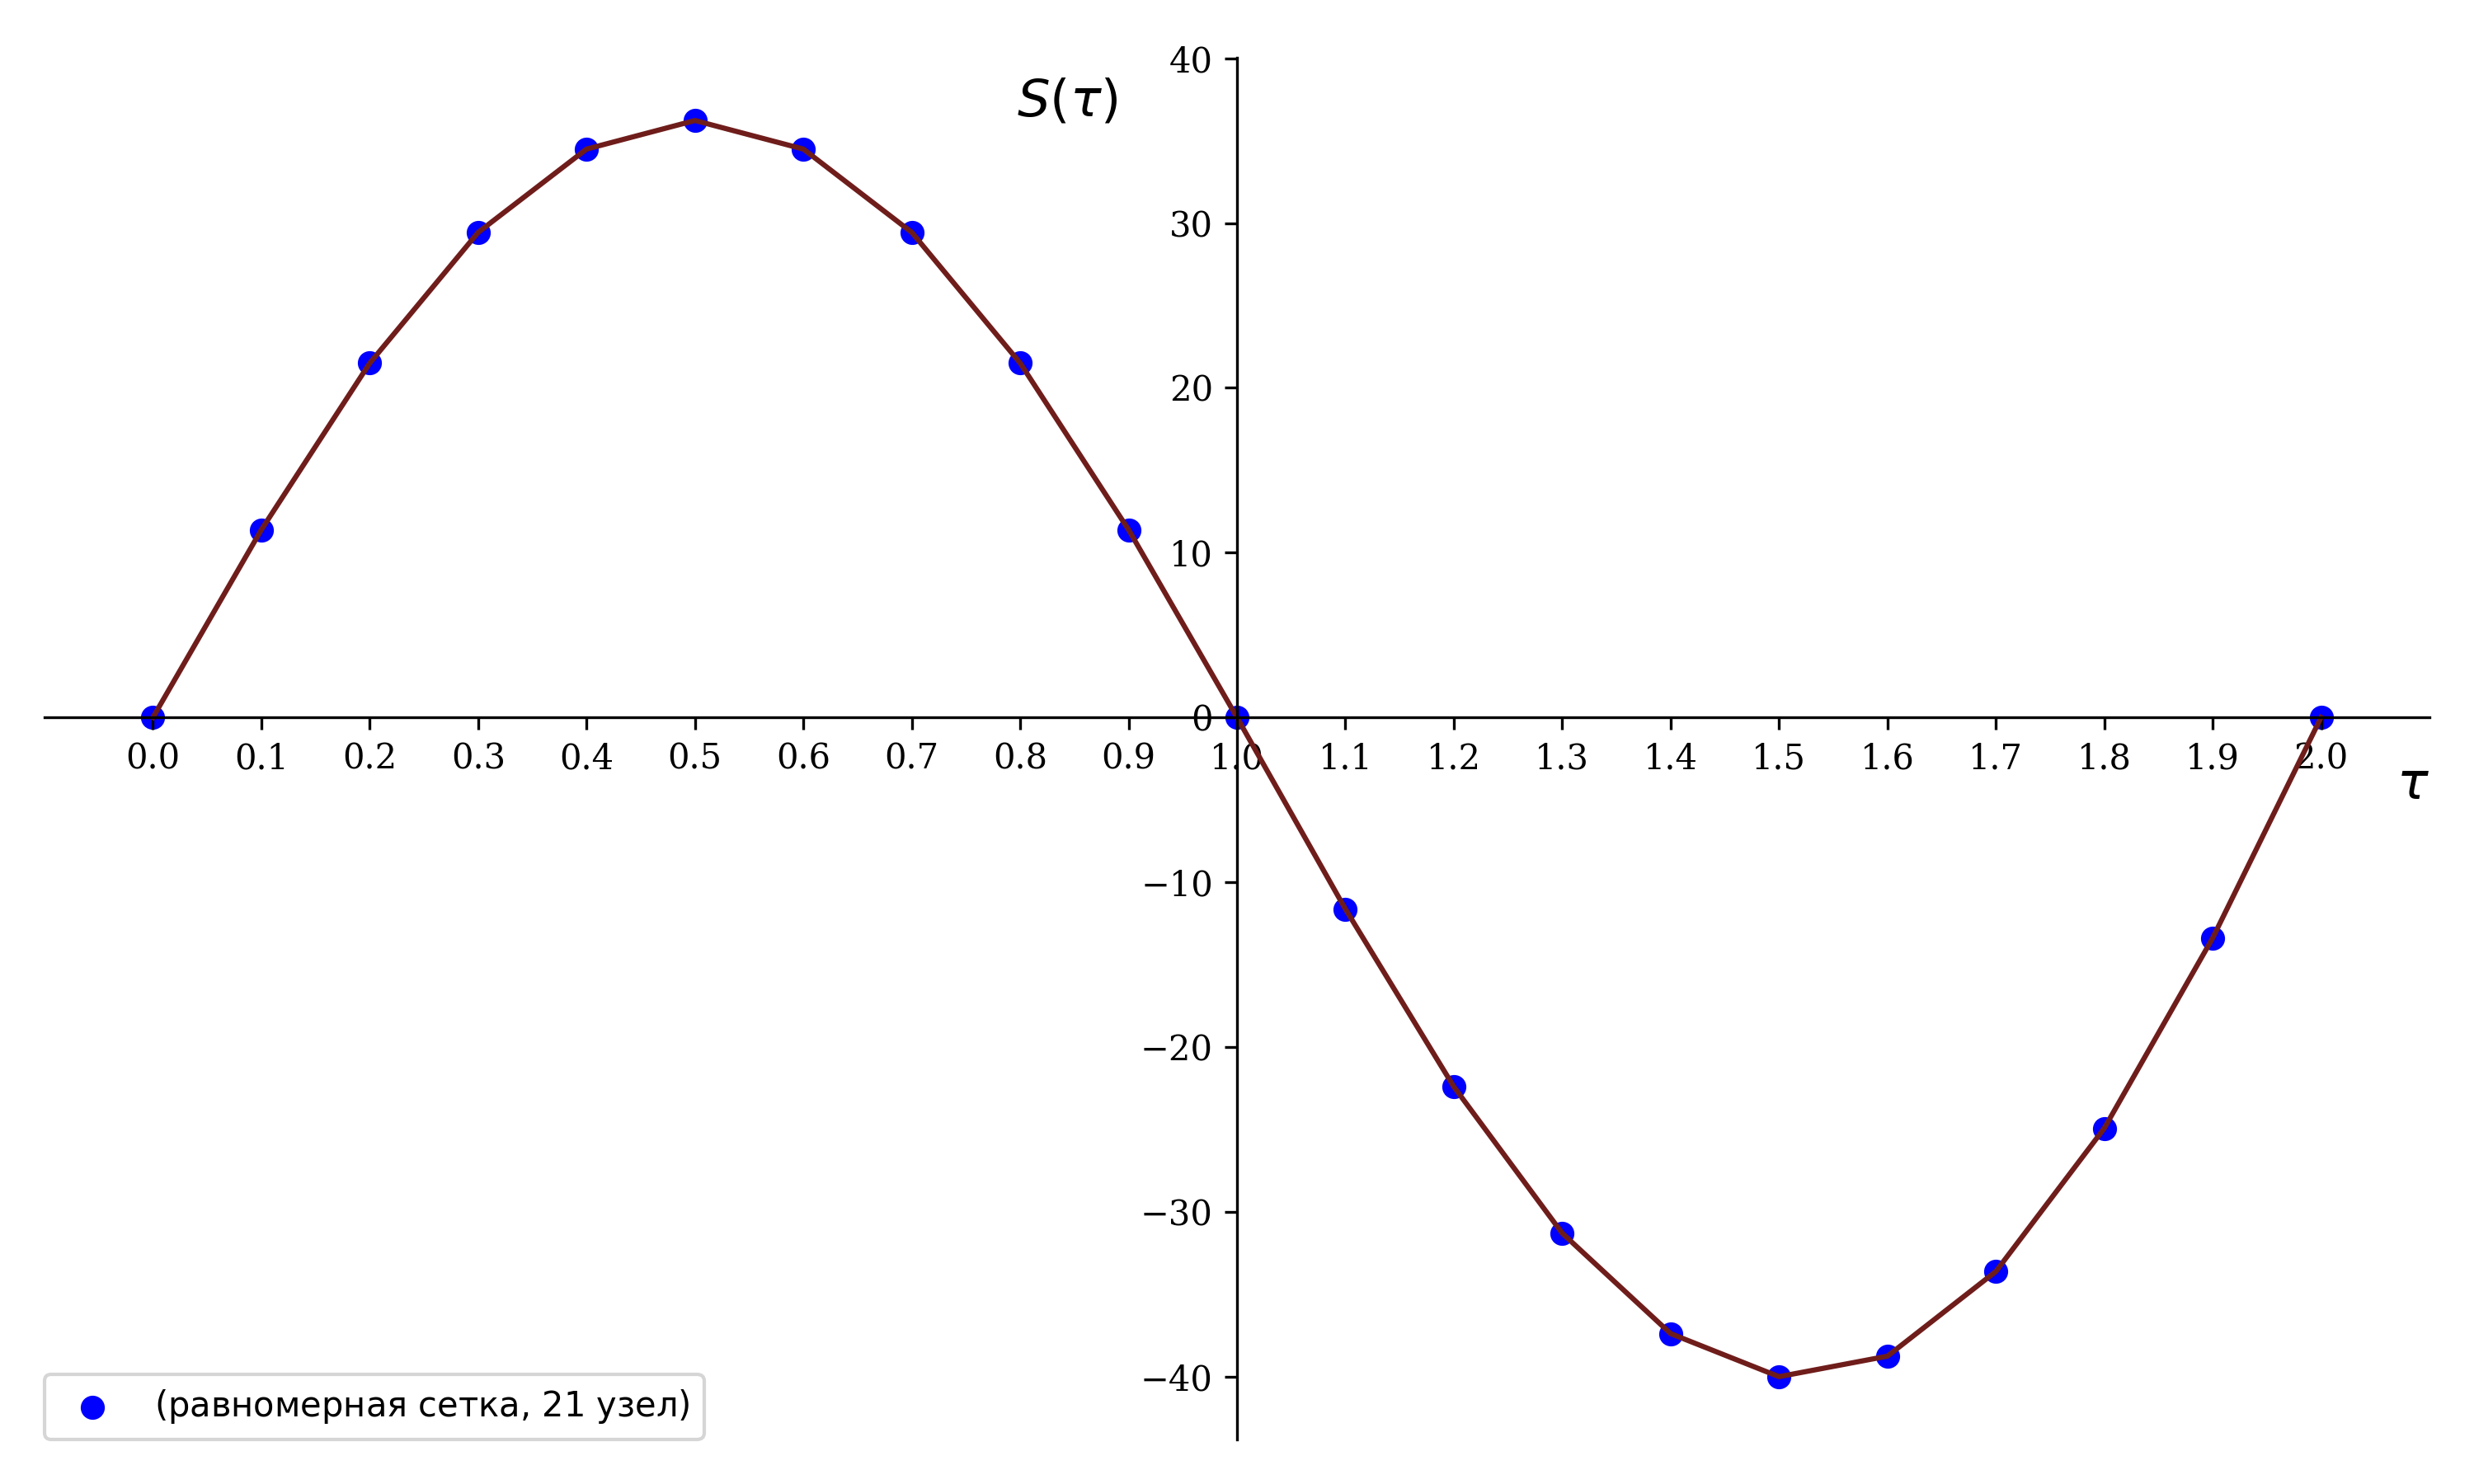
\includegraphics[width=0.85\textwidth]{spline_20}
\end{center}


Теперь построим совмещенные графики заданной функции $f(\tau)$ (точки) и 
найденного сплайна $S(\tau)$:

\begin{center}
    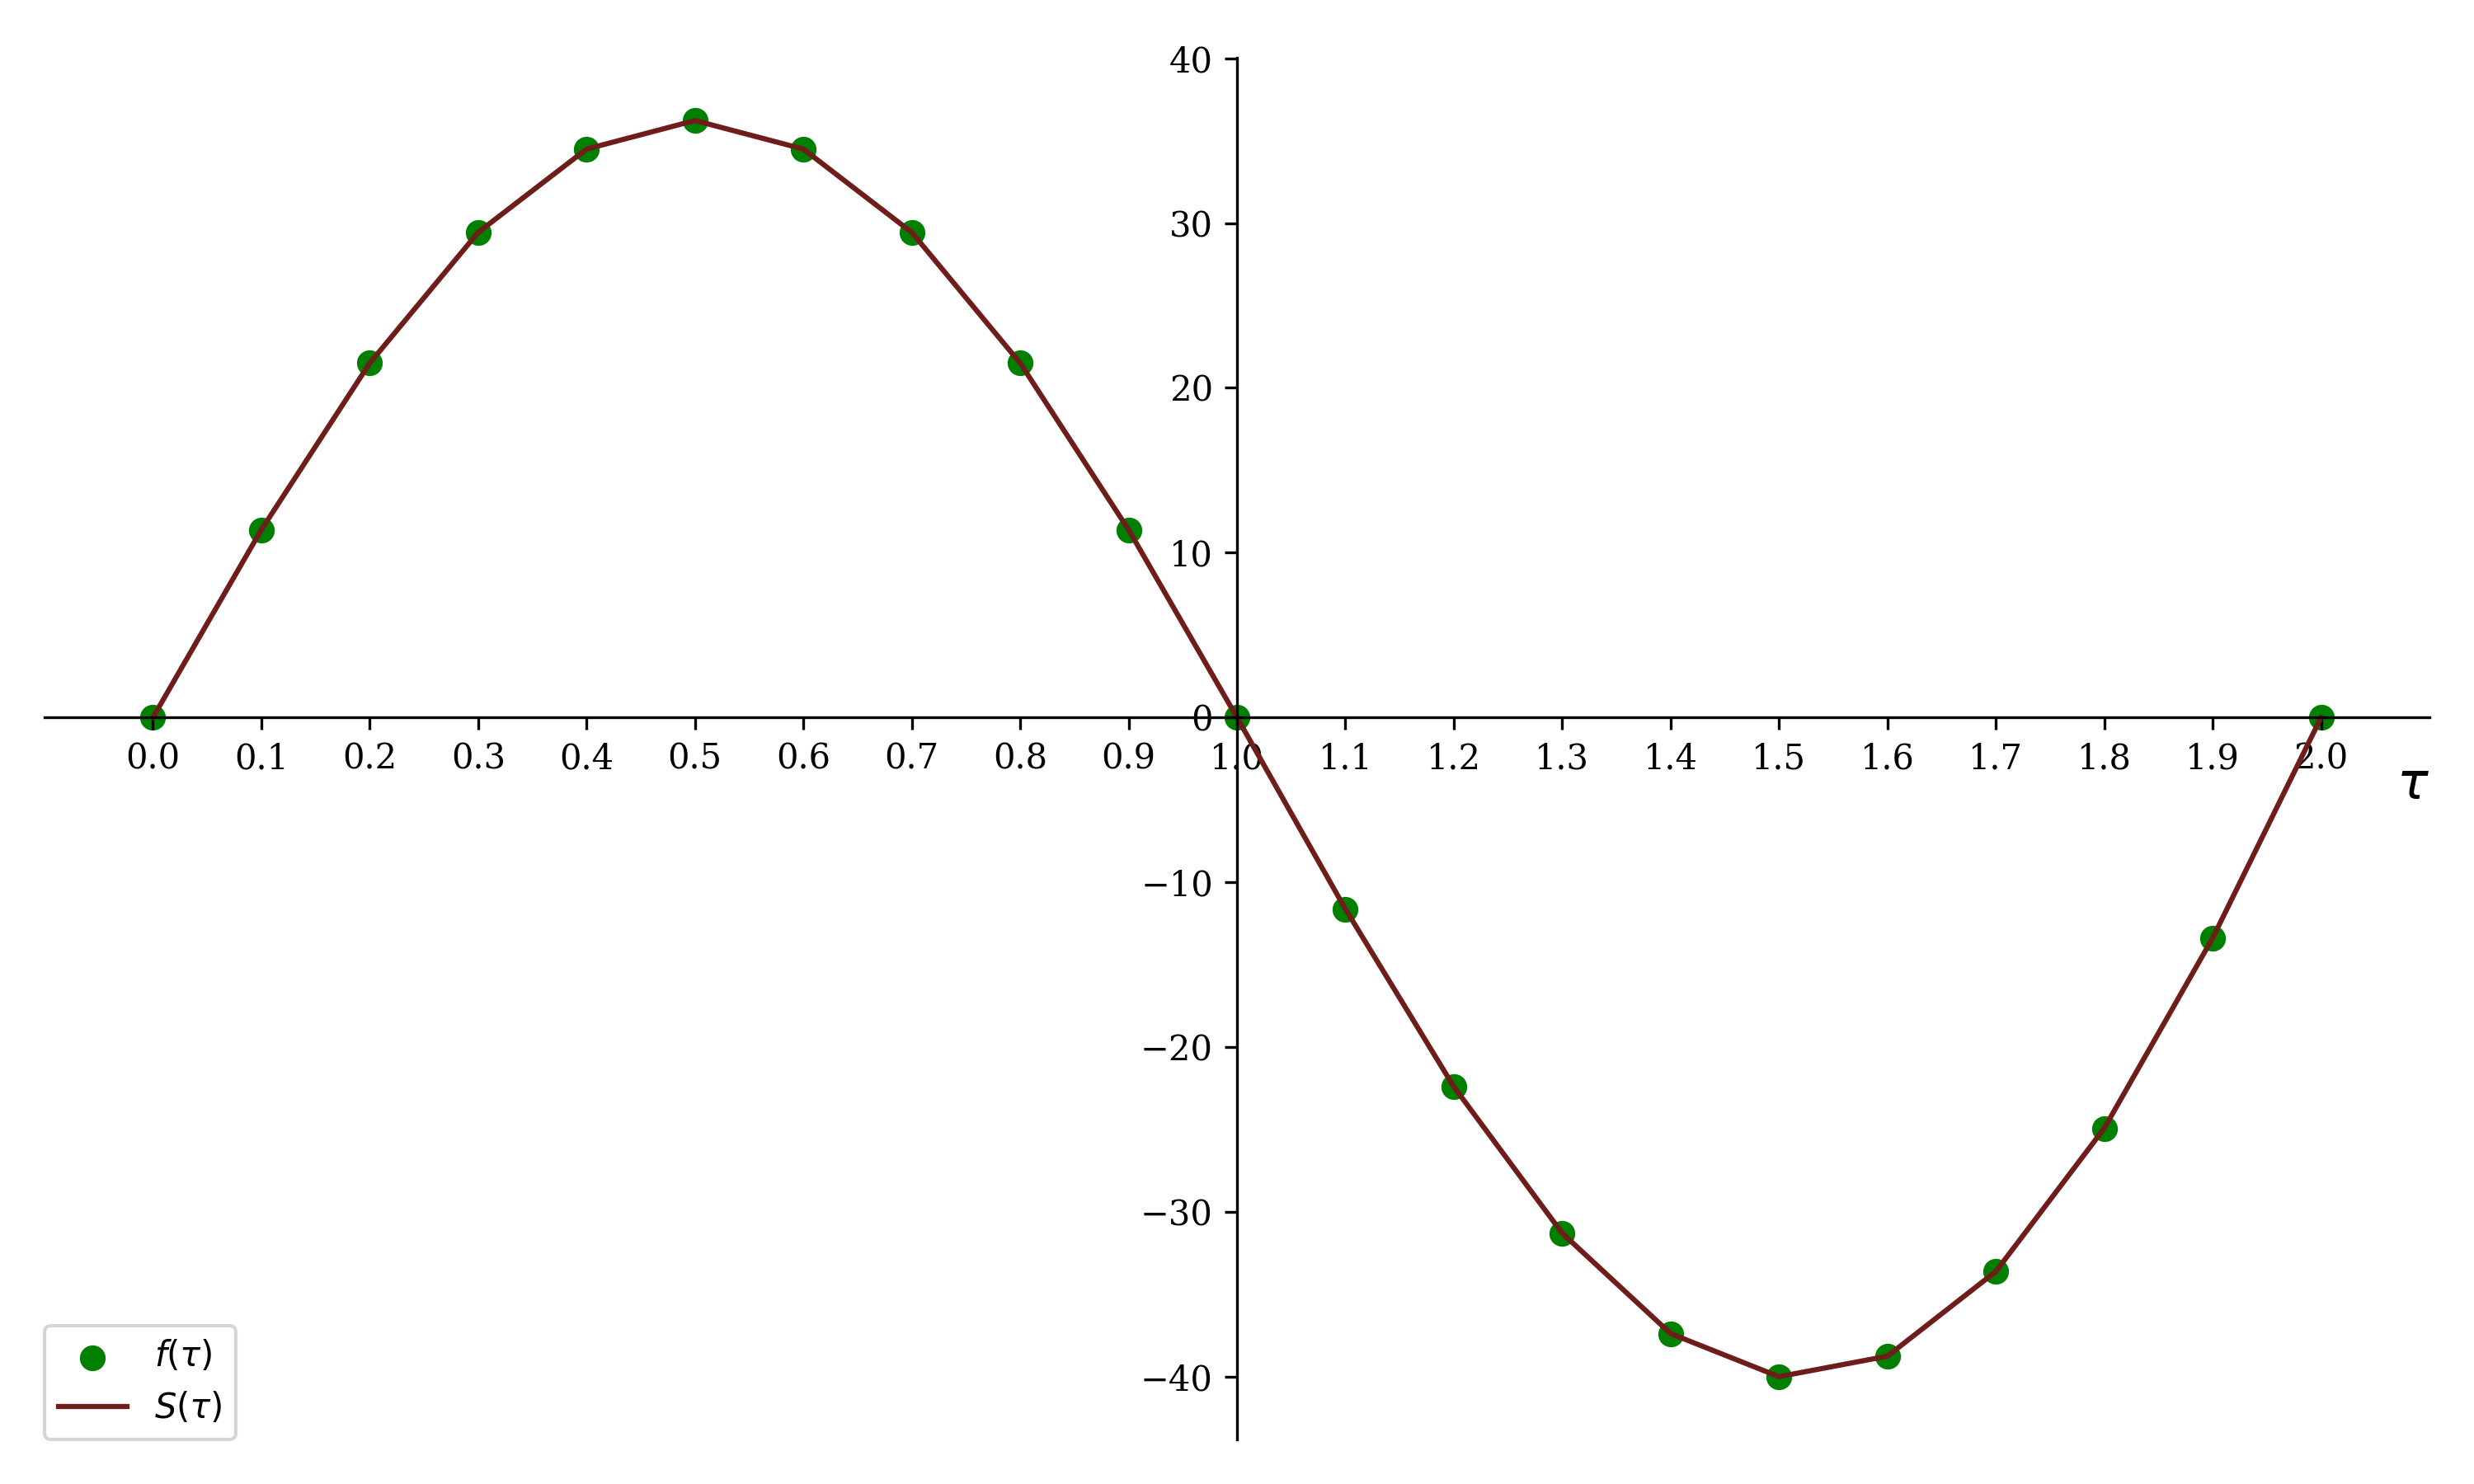
\includegraphics[width=0.85\textwidth]{main_x_spline_20.png}
\end{center}

В качестве проверки, проведем все вышеописанные действия для равномерной сетки с 
41м узлом:

\begin{multicols}{3}
    \begin{enumerate}[itemsep=5pt]
        \item (x: 0.0, y: 0.0)
        \item (x: 0.05, y: 5.791)
        \item (x: 0.1, y: 11.388)
        \item (x: 0.15, y: 16.664)
        \item (x: 0.2, y: 21.5)
        \item (x: 0.25, y: 25.788)
        \item (x: 0.3, y: 29.432)
        \item (x: 0.35, y: 32.353)
        \item (x: 0.4, y: 34.487)
        \item (x: 0.45, y: 35.785)
        \item (x: 0.5, y: 36.222)
        \item (x: 0.55, y: 35.785)
        \item (x: 0.6, y: 34.487)
        \item (x: 0.65, y: 32.353)
        \item (x: 0.7, y: 29.432)
        \item (x: 0.75, y: 25.788)
        \item (x: 0.8, y: 21.5)
        \item (x: 0.85, y: 16.664)
        \item (x: 0.9, y: 11.388)
        \item (x: 0.95, y: 5.791)
        \item (x: 1.0, y: 0.0)
        \item (x: 1.05, y: -5.851)
        \item (x: 1.1, y: -11.627)
        \item (x: 1.15, y: -17.19)
        \item (x: 1.2, y: -22.406)
        \item (x: 1.25, y: -27.148)
        \item (x: 1.3, y: -31.295)
        \item (x: 1.35, y: -34.739)
        \item (x: 1.4, y: -37.386)
        \item (x: 1.45, y: -39.159)
        \item (x: 1.5, y: -40.0)
        \item (x: 1.55, y: -39.87)
        \item (x: 1.6, y: -38.755)
        \item (x: 1.65, y: -36.66)
        \item (x: 1.7, y: -33.618)
        \item (x: 1.75, y: -29.682)
        \item (x: 1.8, y: -24.929)
        \item (x: 1.85, y: -19.458)
        \item (x: 1.9, y: -13.386)
        \item (x: 1.95, y: -6.85)
        \item (x: 2.0, y: -0.0)
    \end{enumerate} 
\end{multicols}

\vfill

Исходная функция:

\begin{center}
    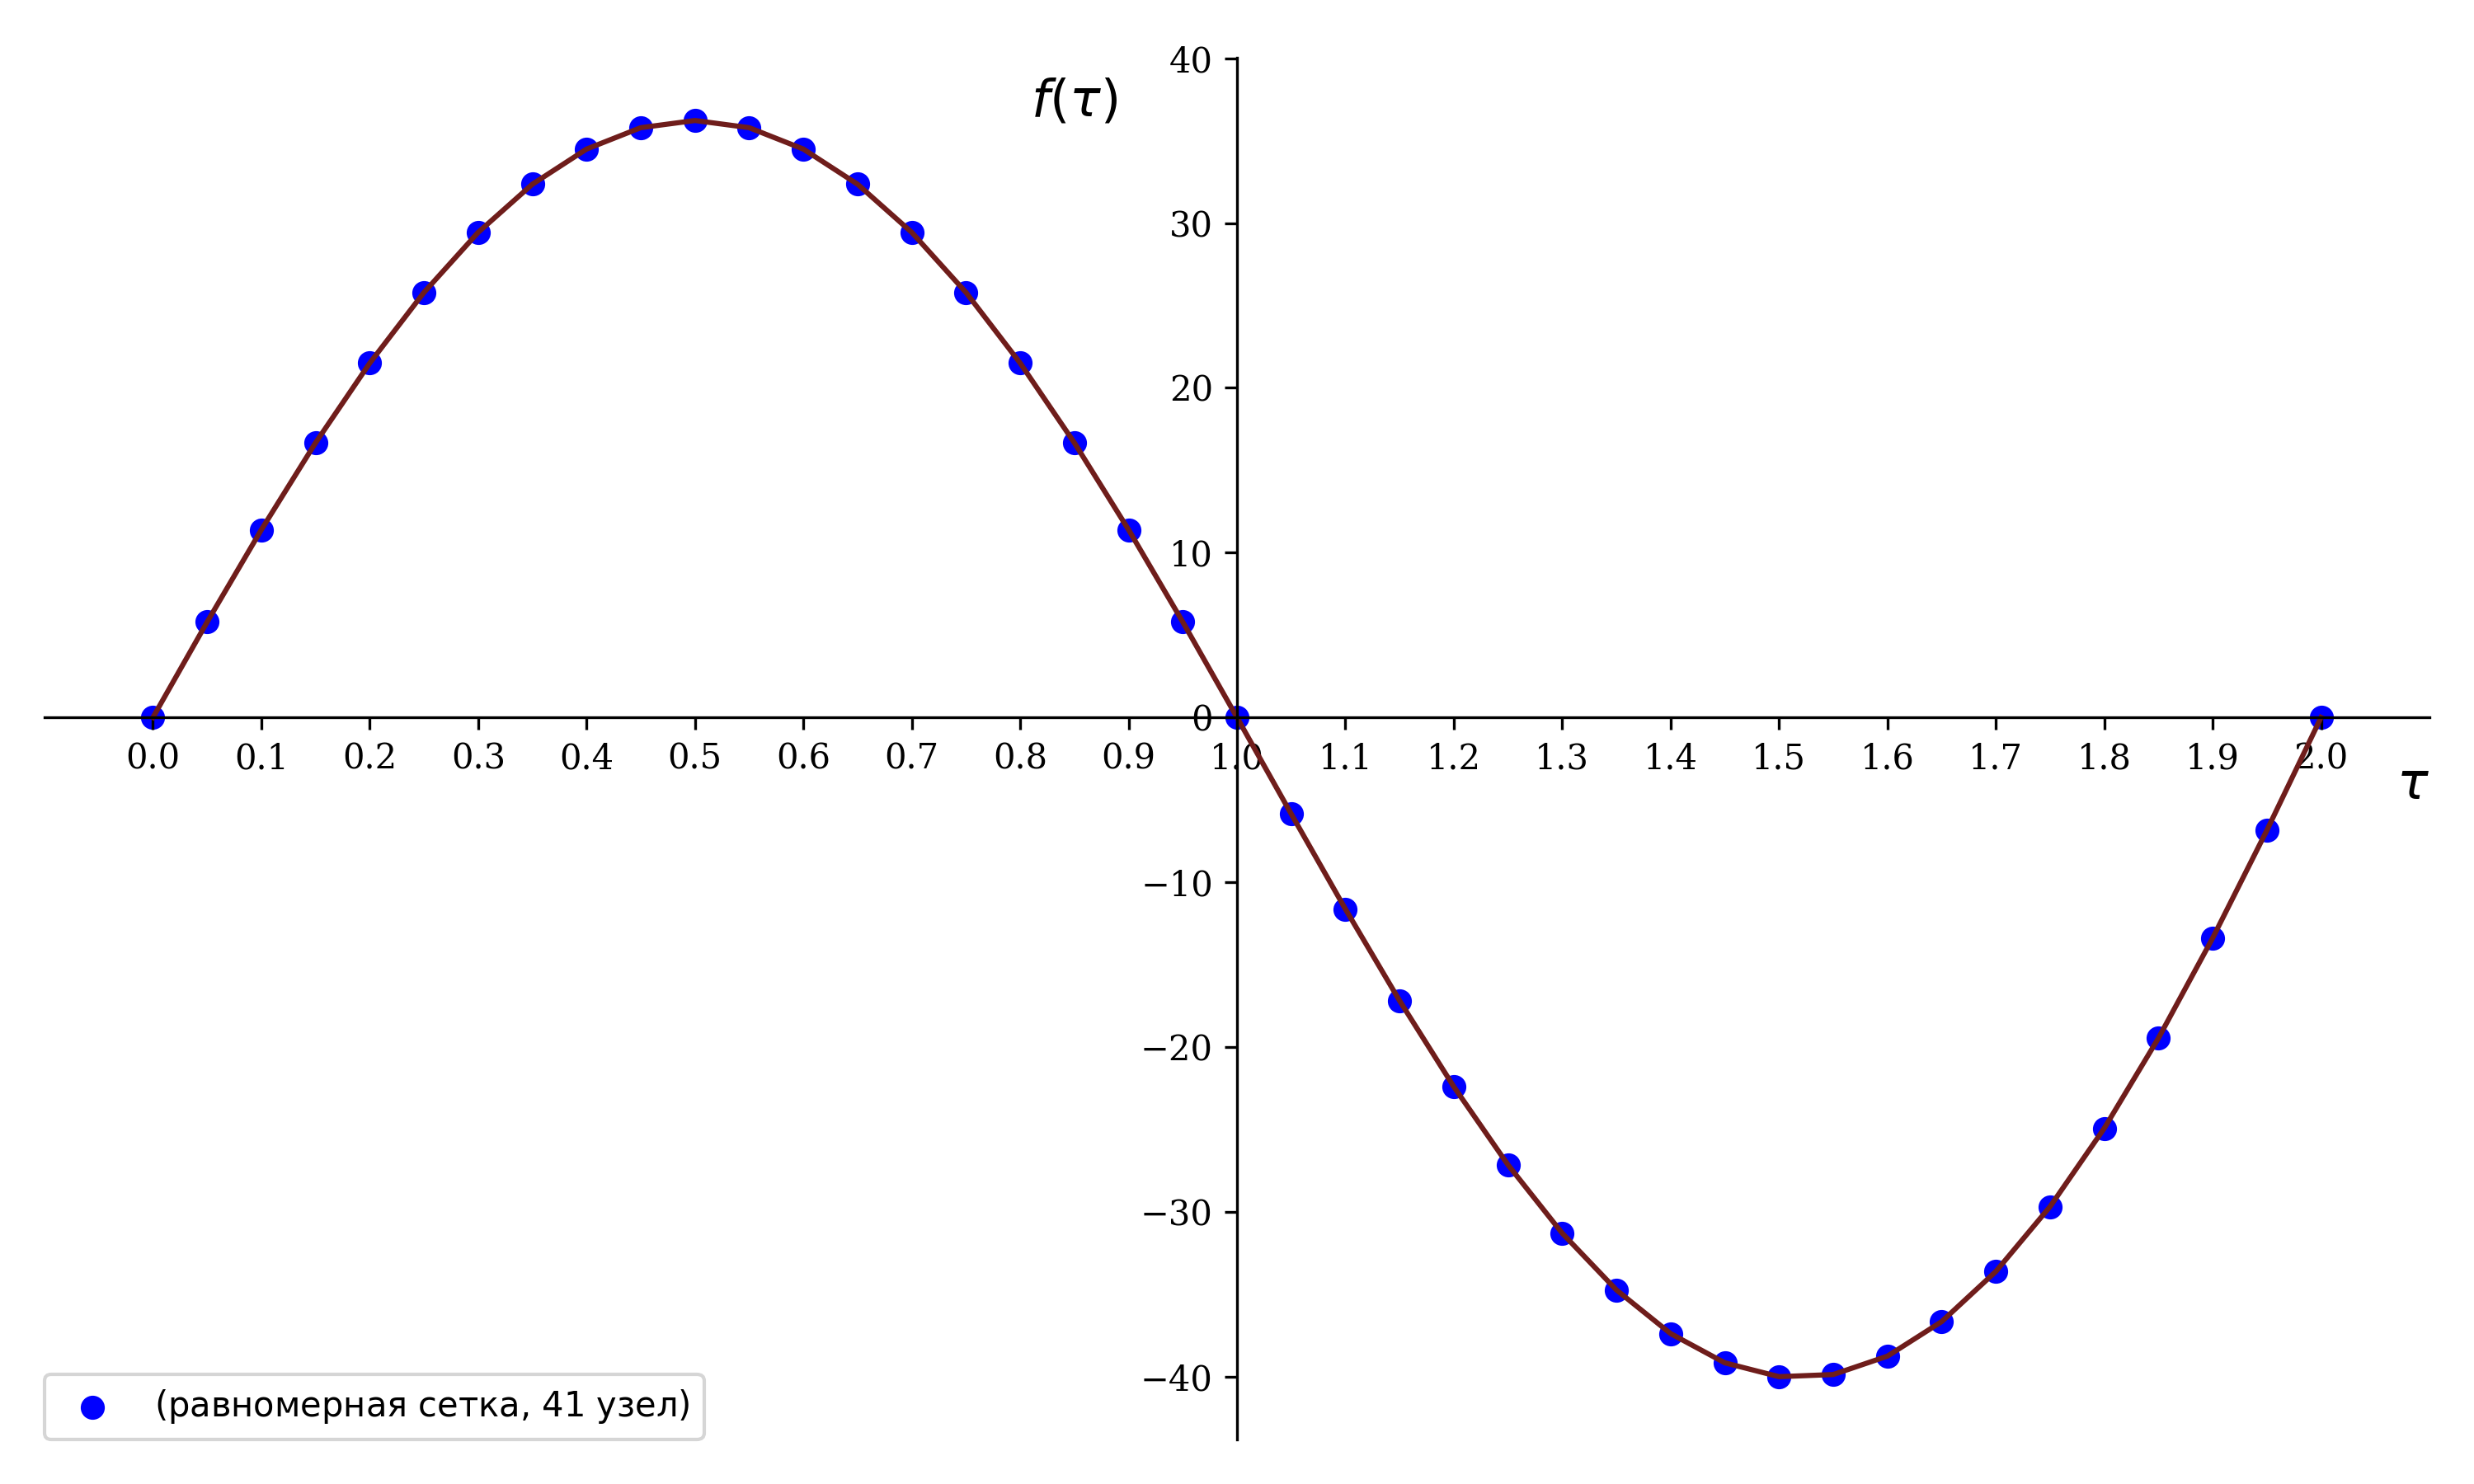
\includegraphics[width=1\textwidth]{main_func_40}
\end{center}

\vfill

\newpage

\vfill

Найденный кубический сплайн: 

\begin{center}
    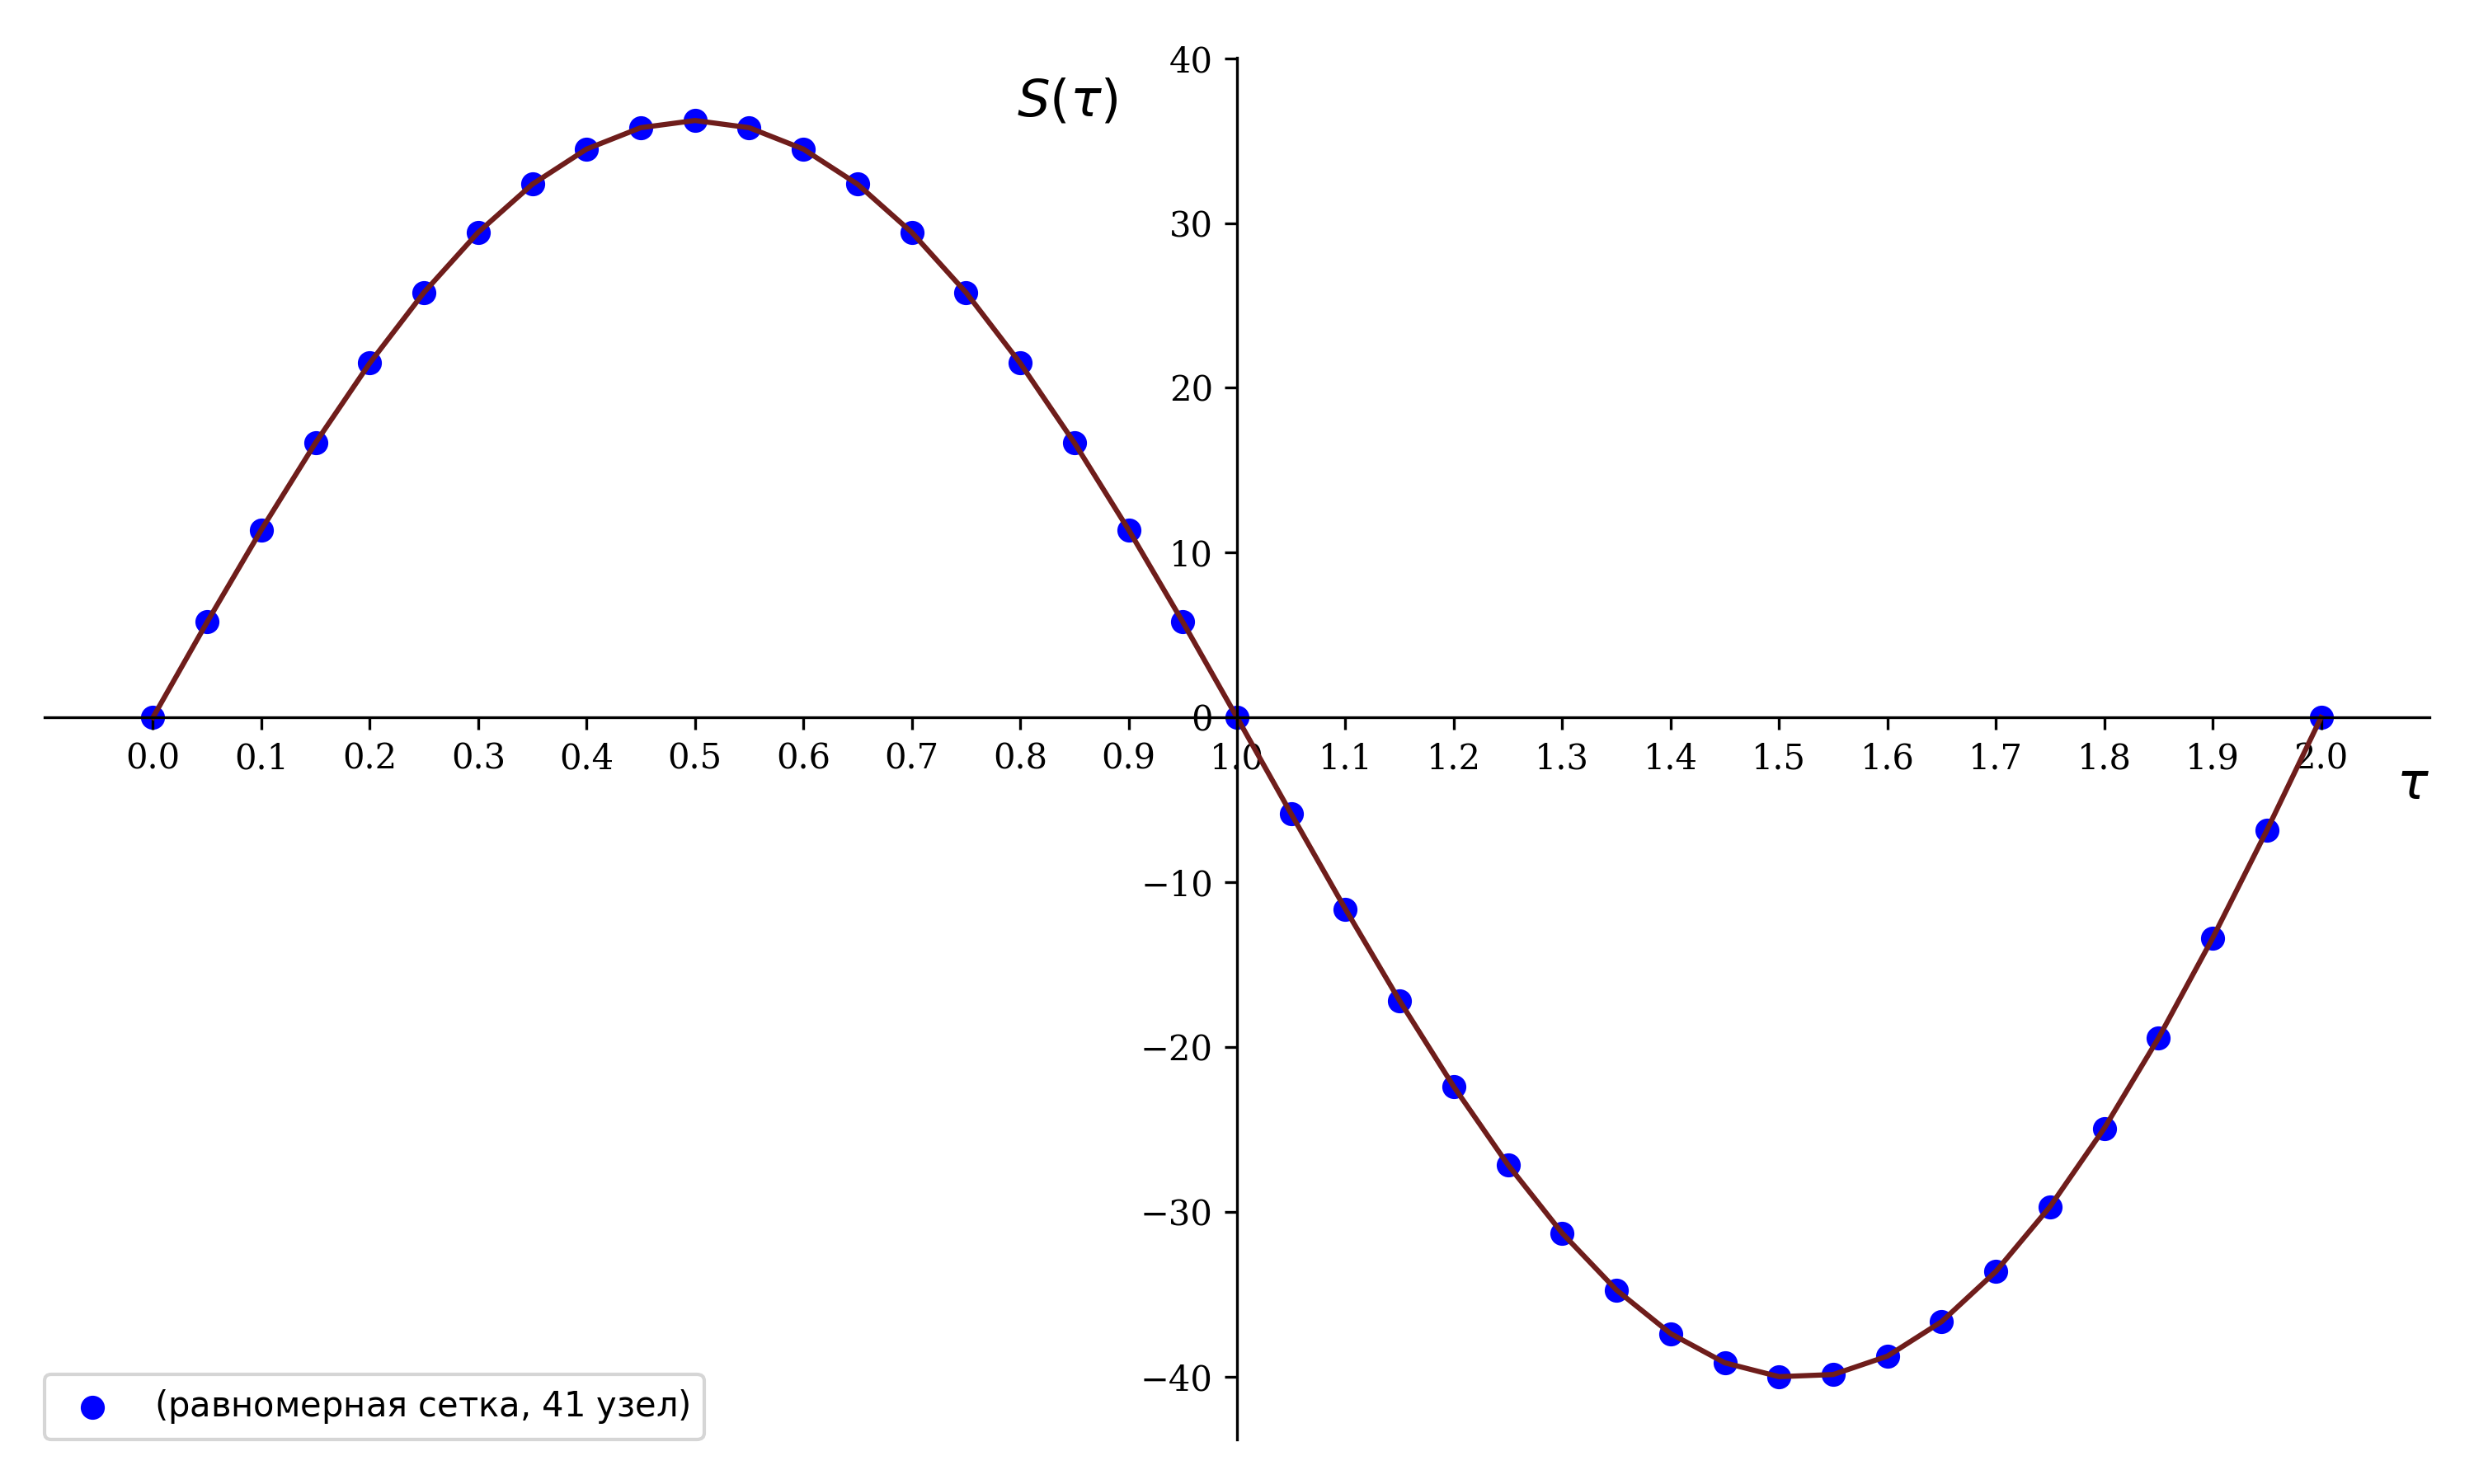
\includegraphics[width=1\textwidth]{spline_40}
\end{center}

Совмещенные графики:

\begin{center}
    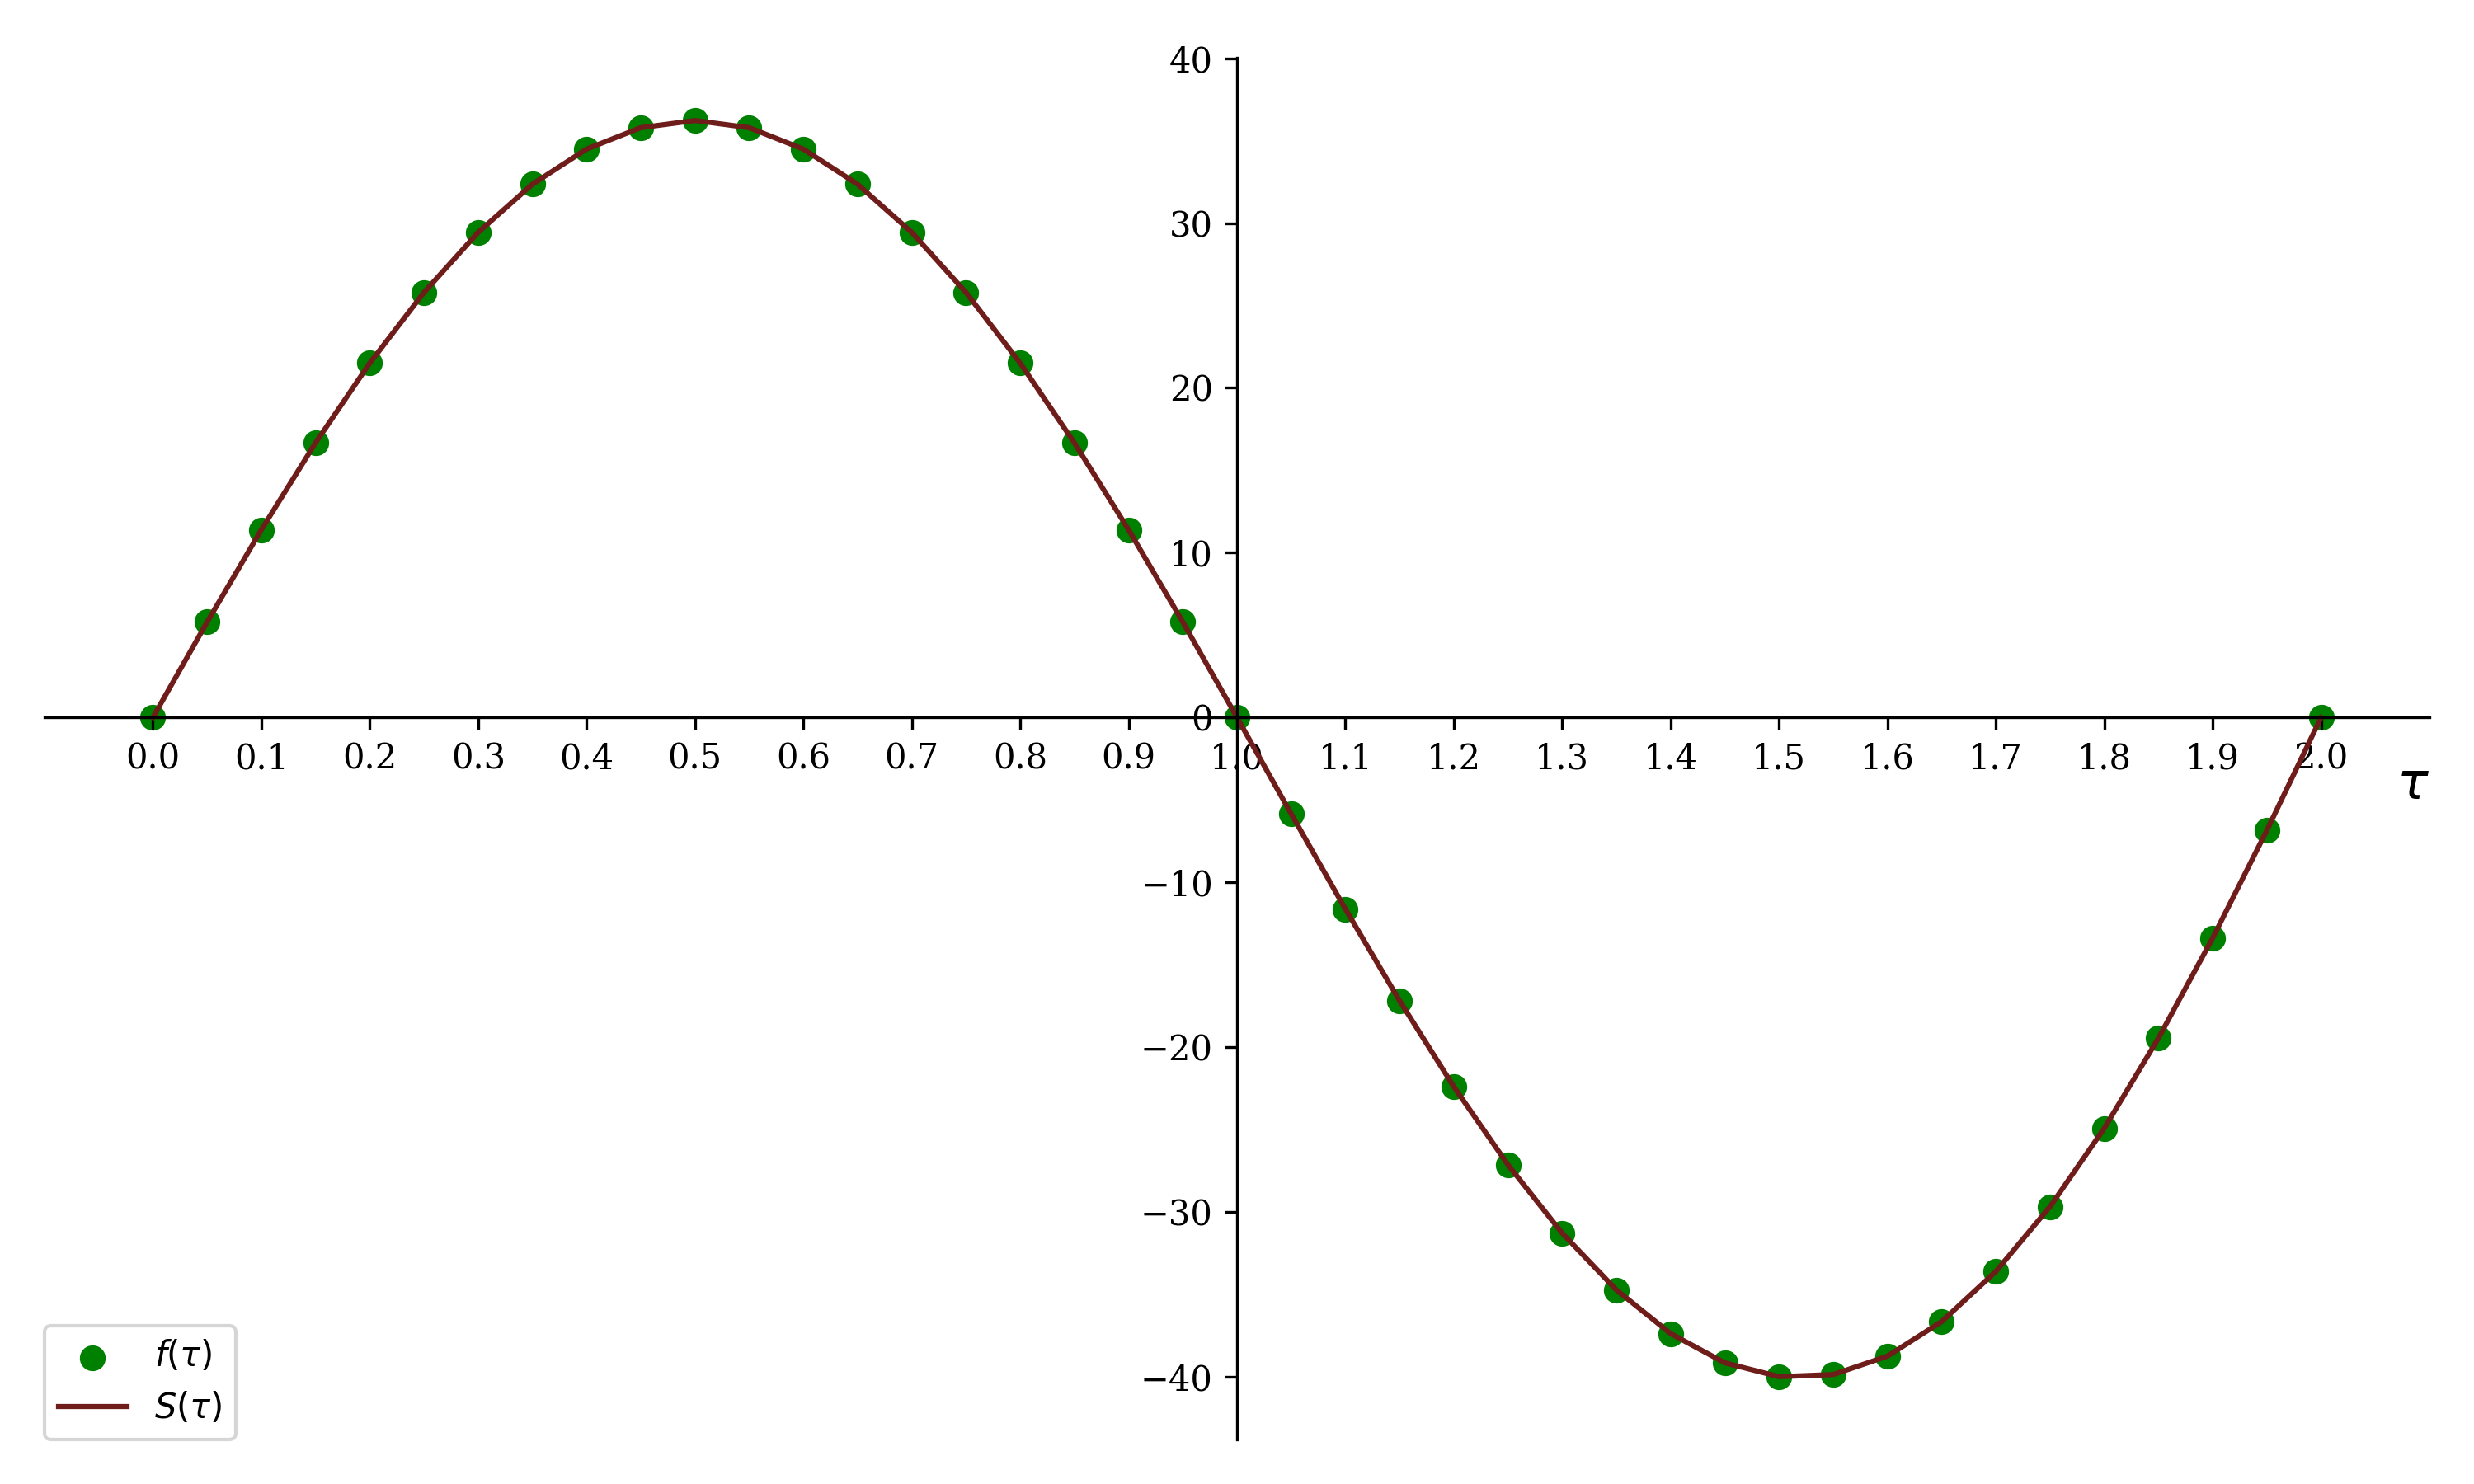
\includegraphics[width=1\textwidth]{main_x_spline_40}
\end{center}

\vfill

А также посмотрим на графики на равномерной сетке со 101 узлом.

\begin{center}
    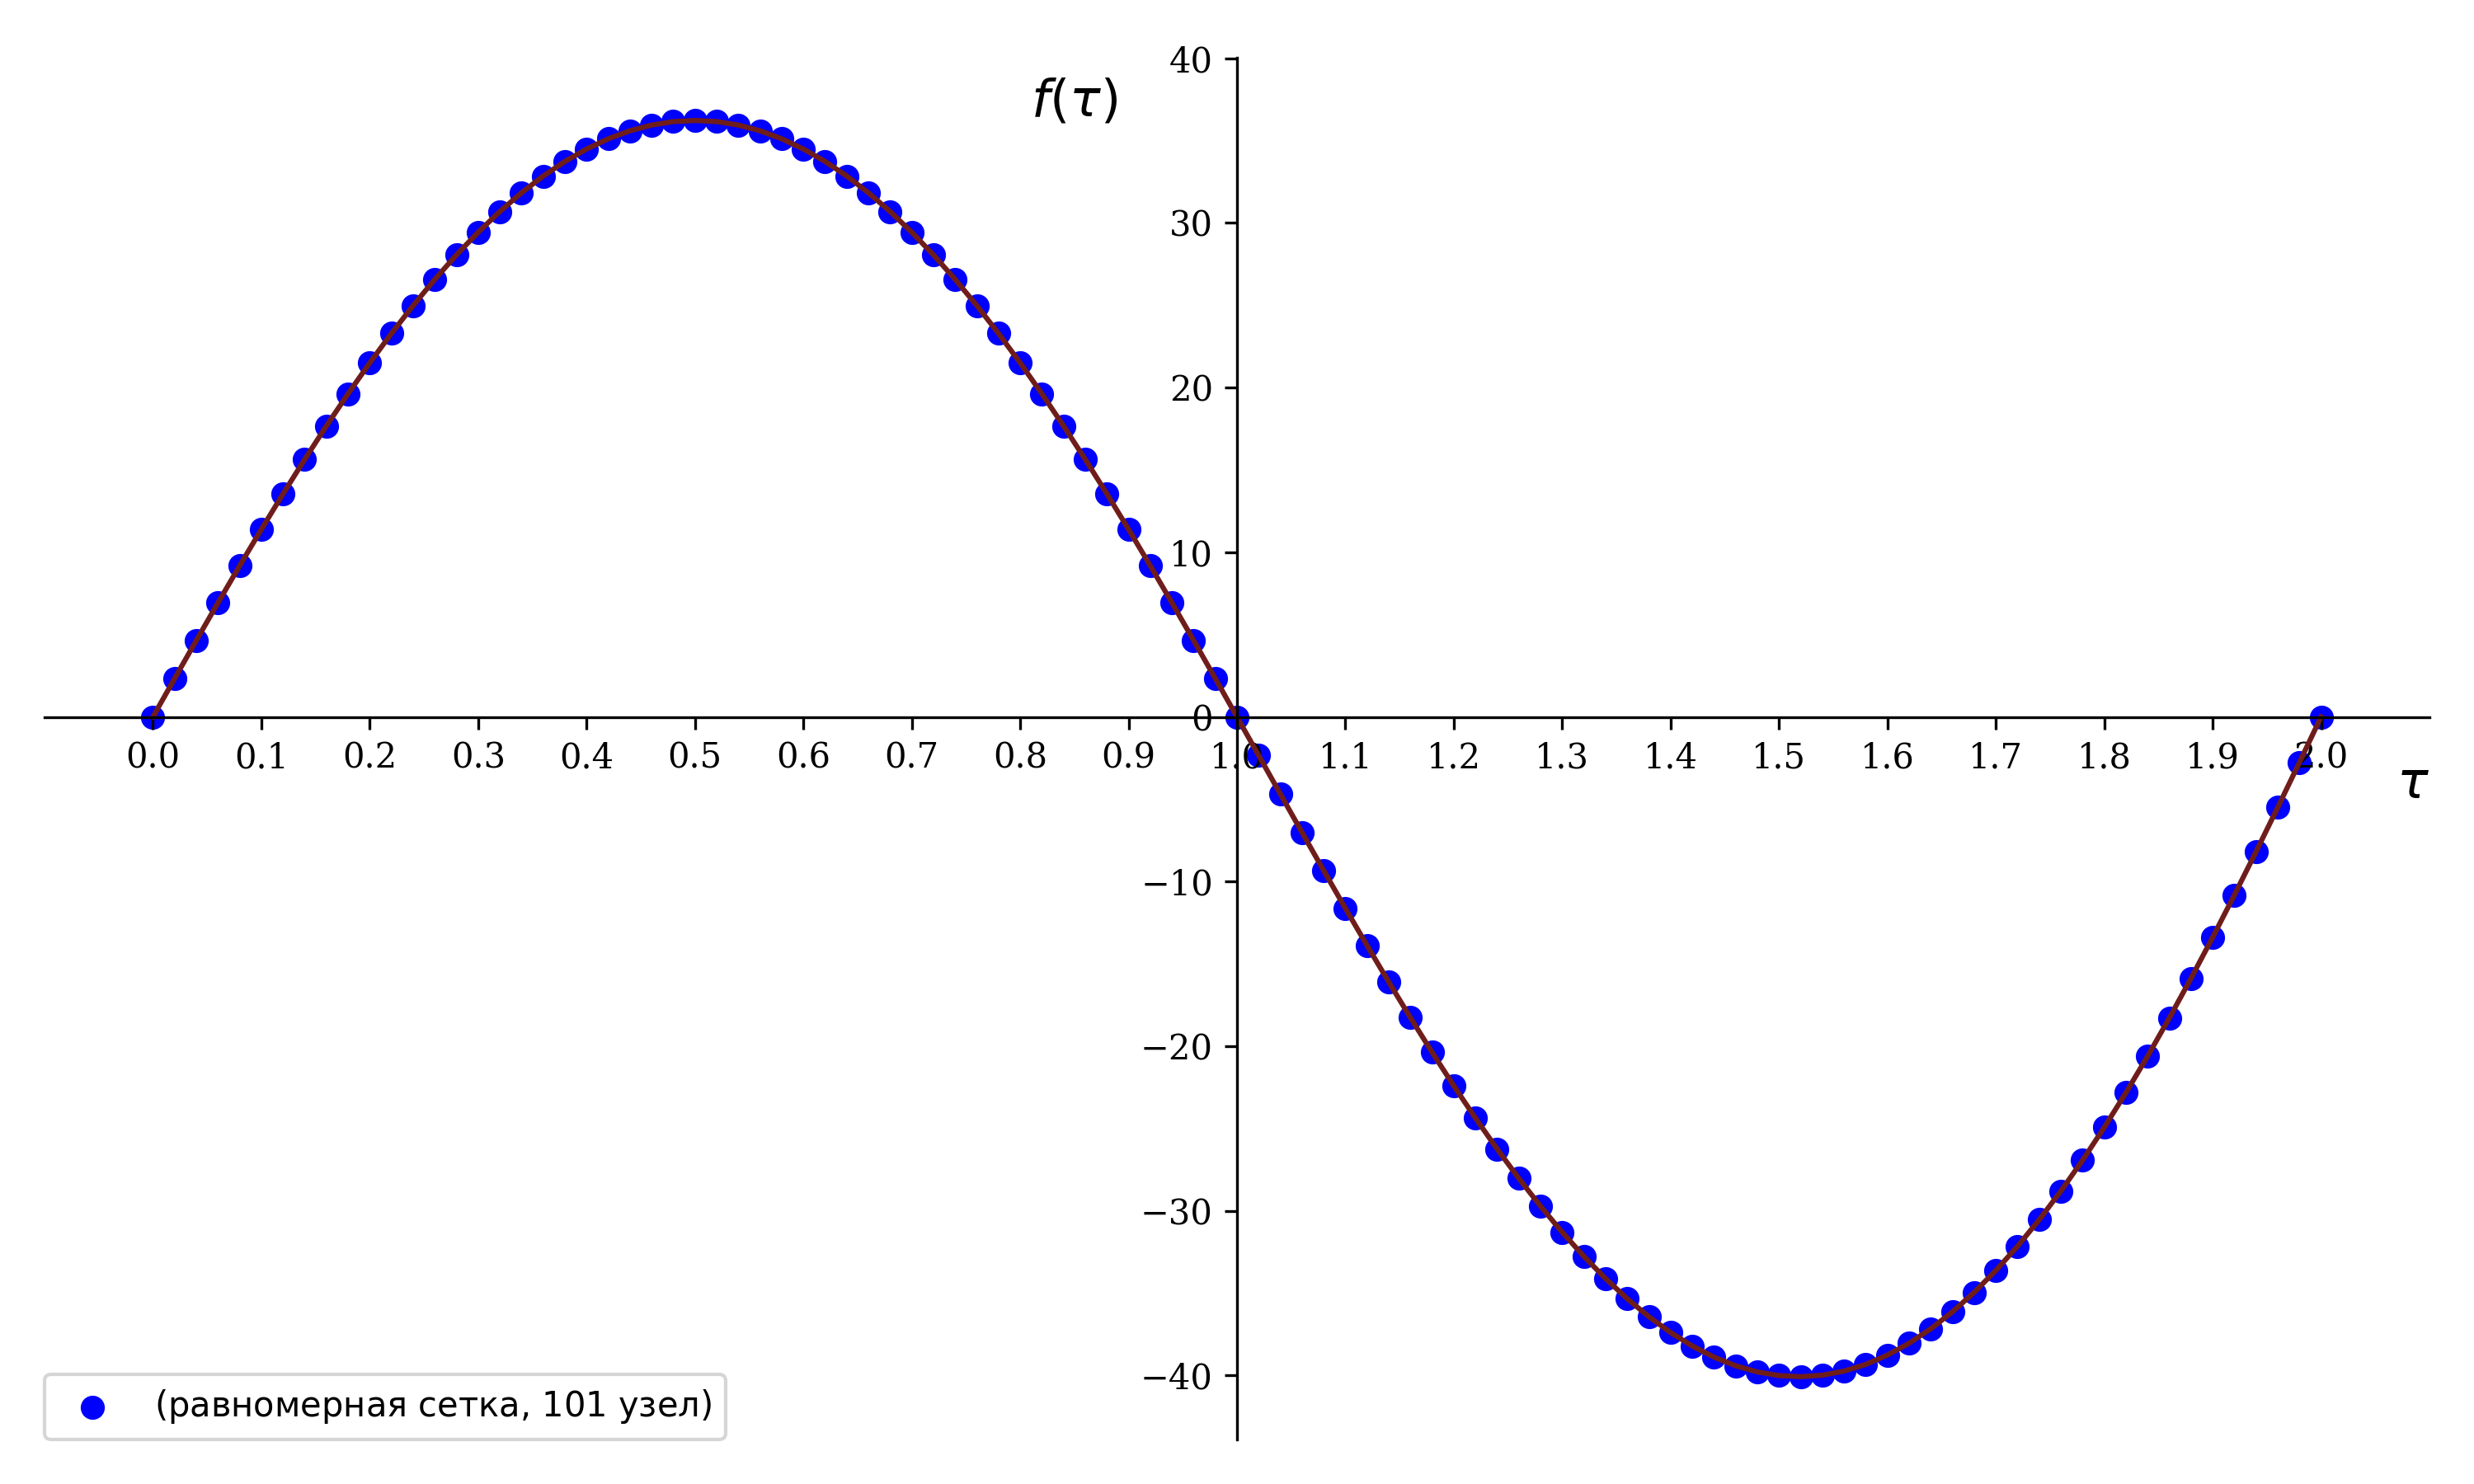
\includegraphics[width=0.85\textwidth]{main_func_100}
\end{center}

\begin{center}
    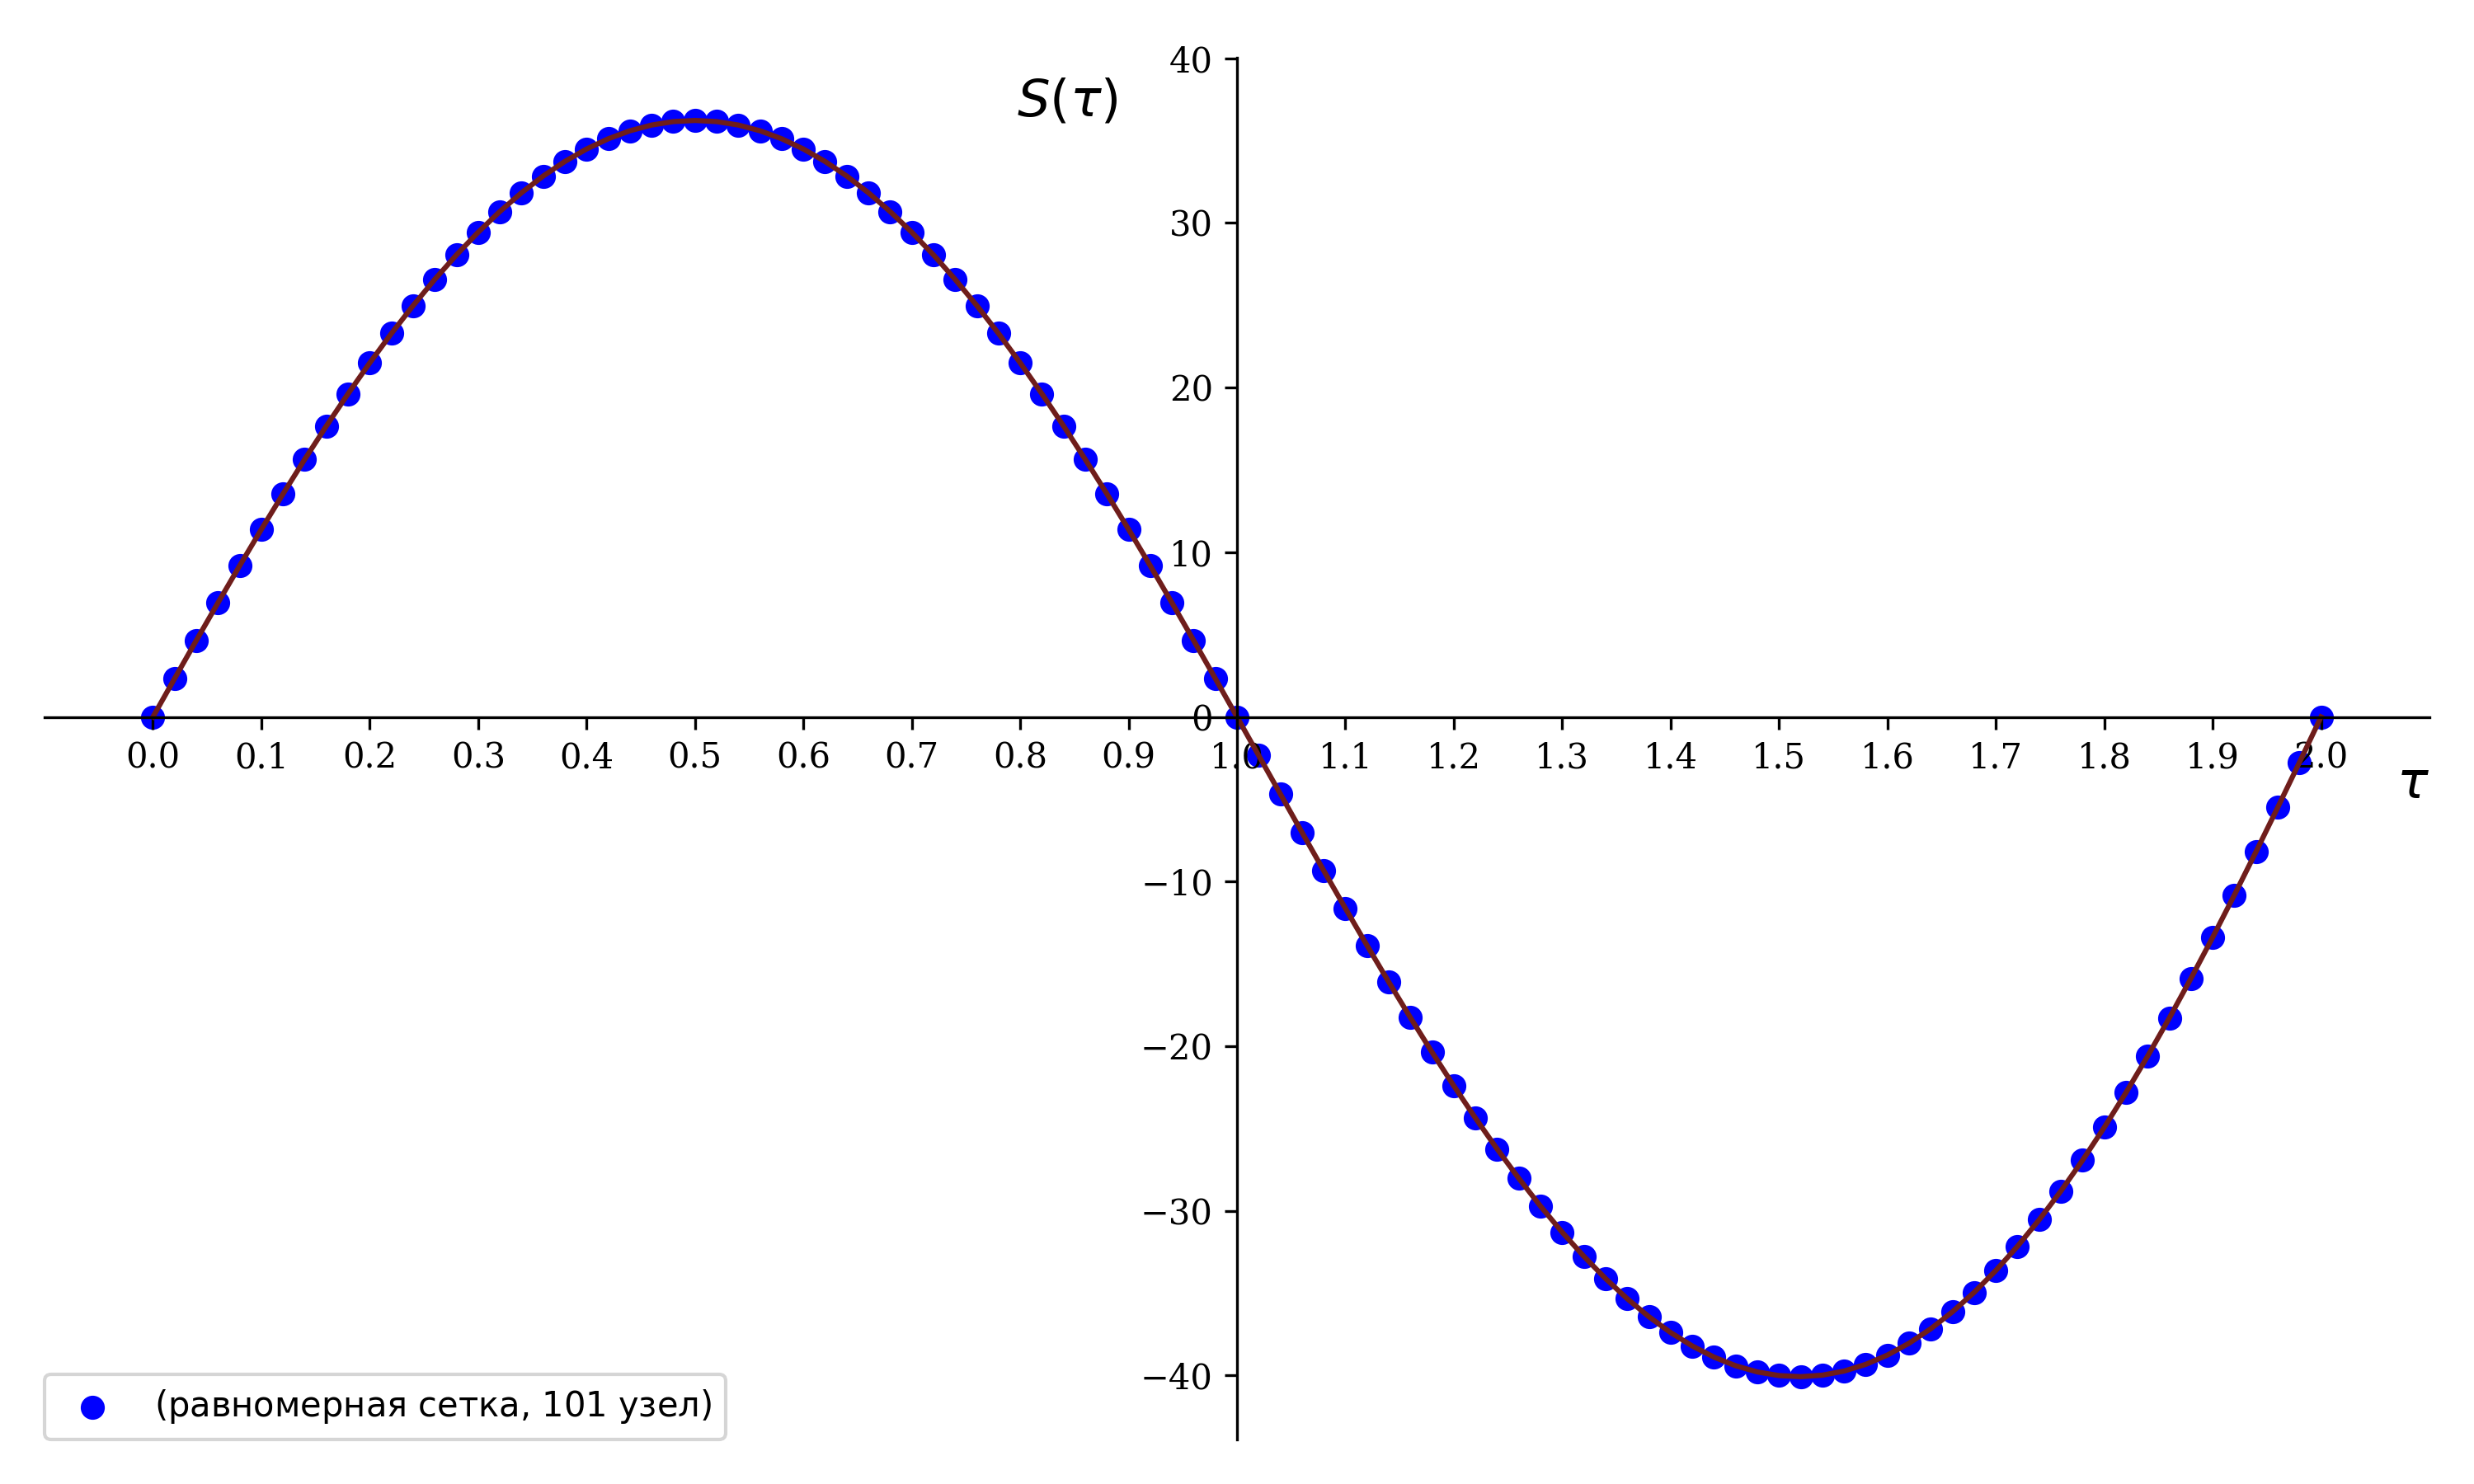
\includegraphics[width=0.85\textwidth]{spline_100}
\end{center}

\begin{center}
    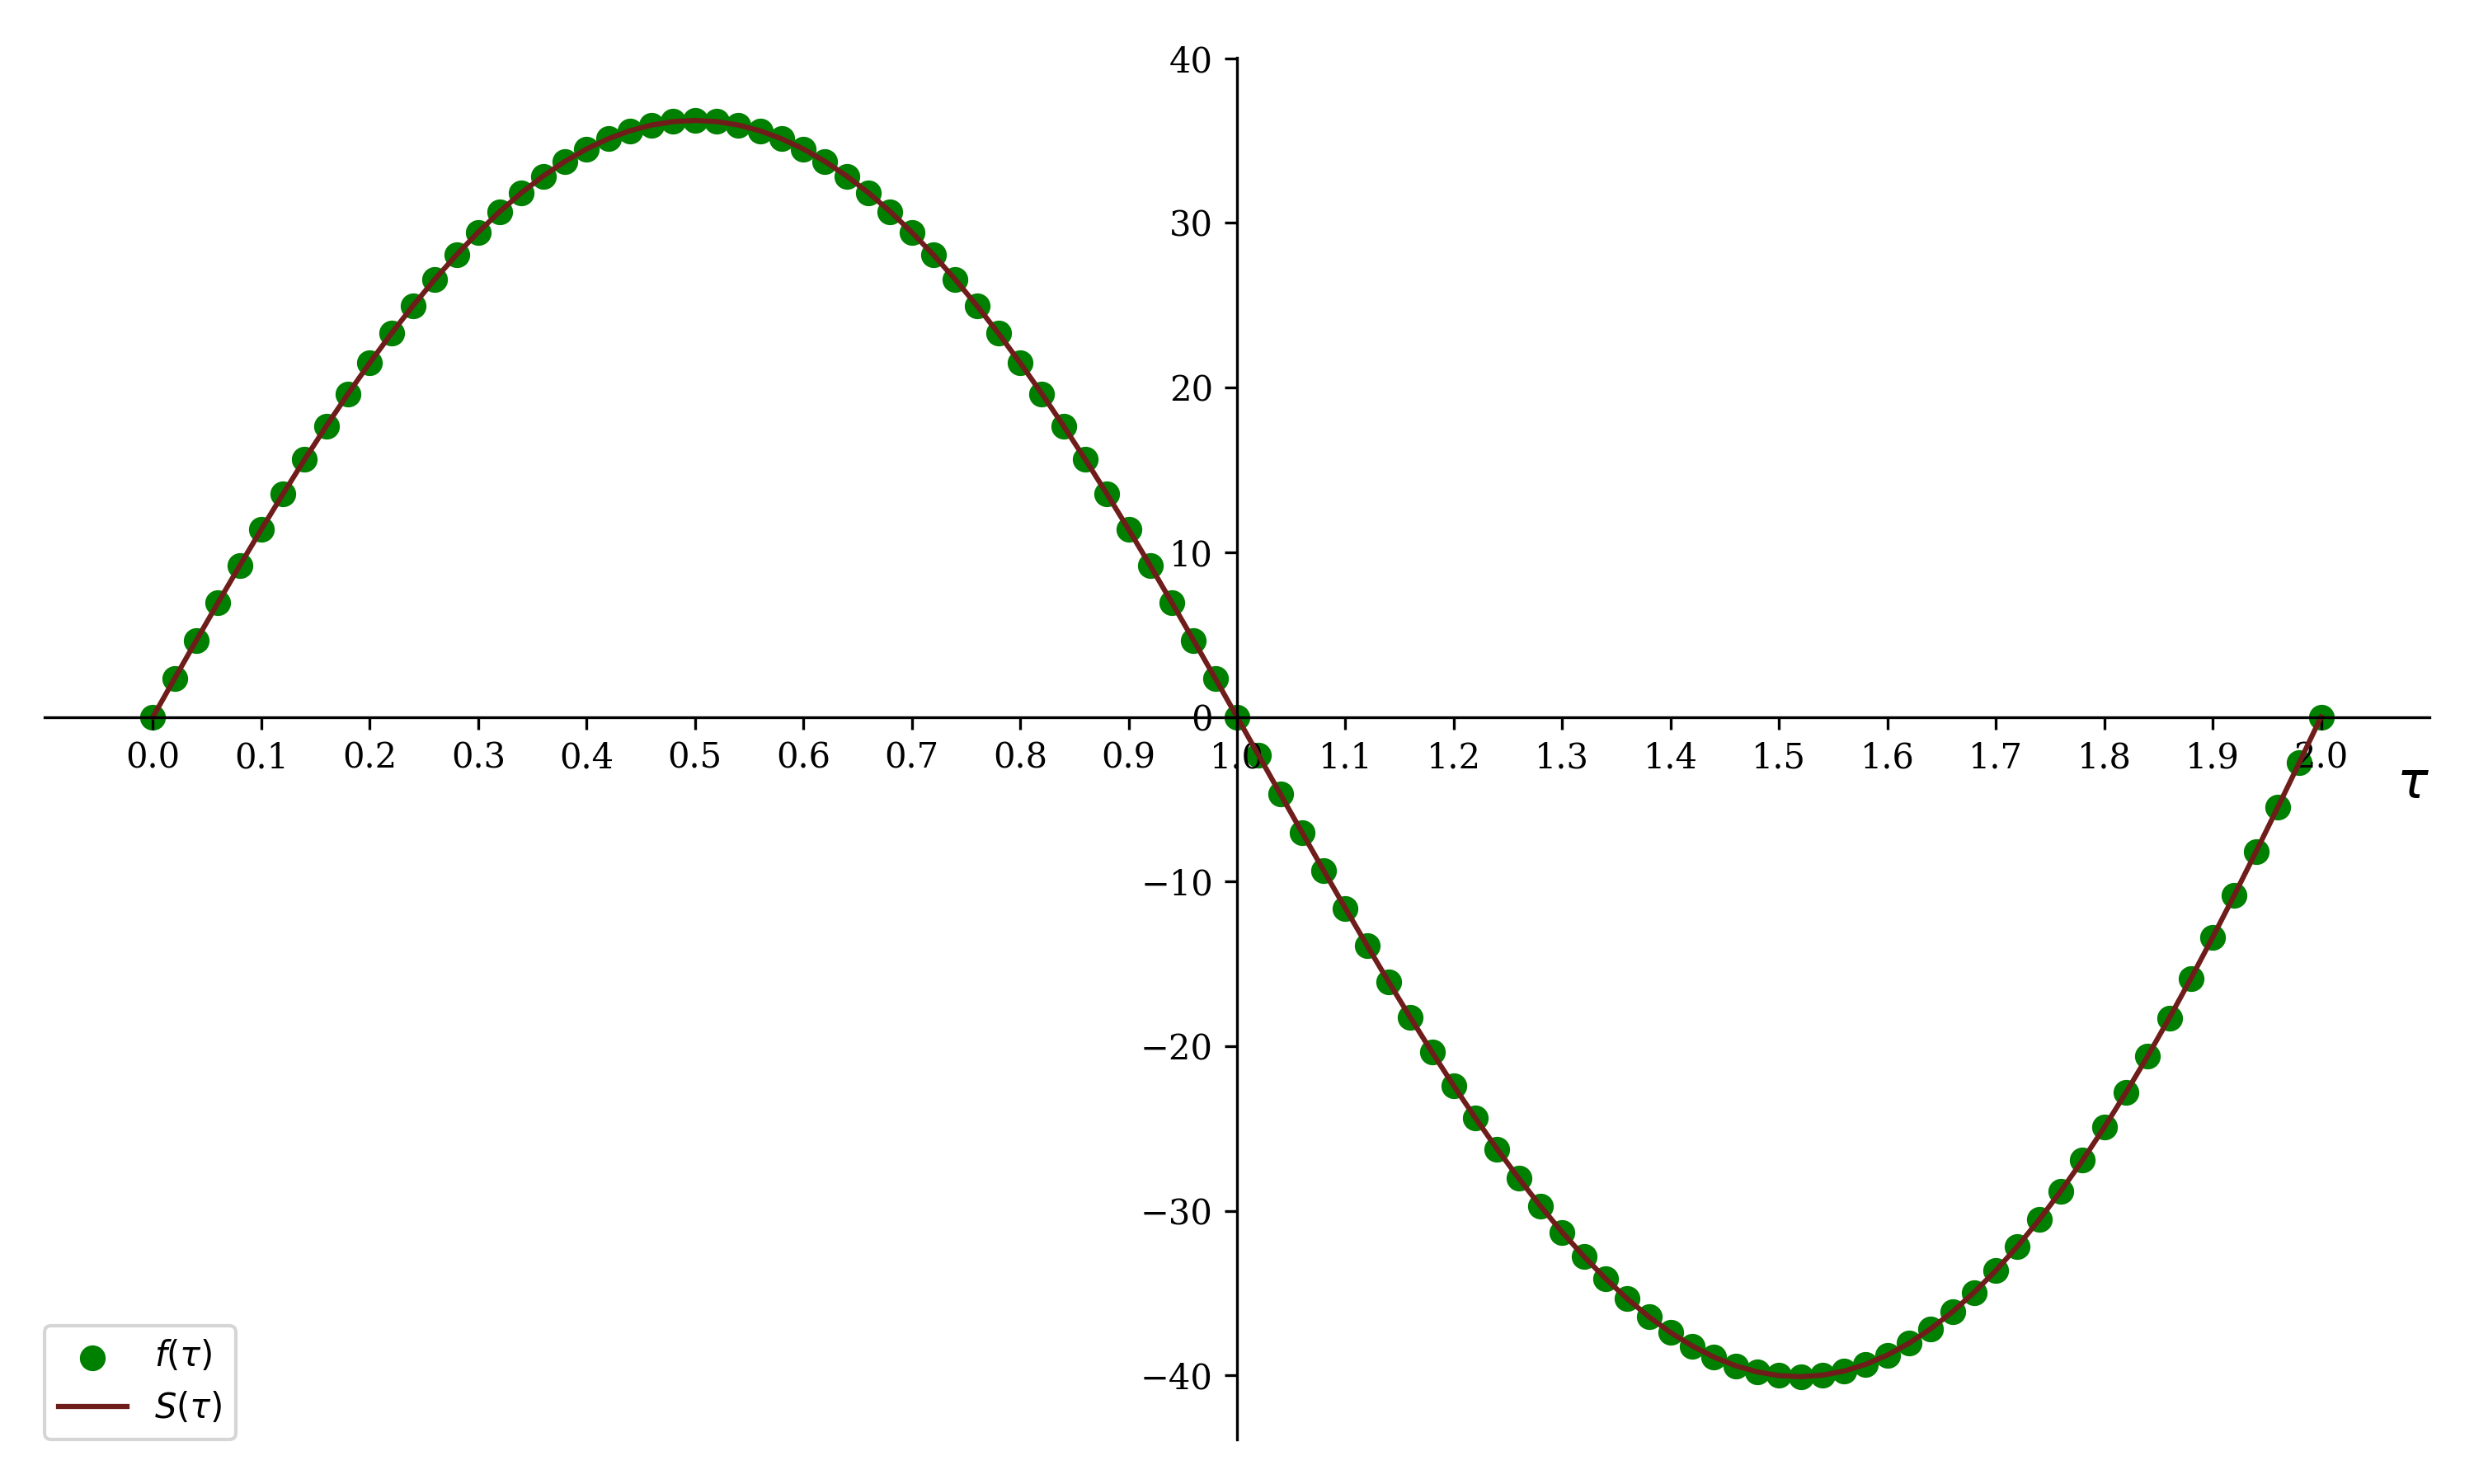
\includegraphics[width=0.85\textwidth]{main_x_spline_100}
\end{center}

Теперь найдем значения производных функций $f(\tau)$ и $S(\tau)$ в узлах равномерной 
сетки при k=20, 40 и 100 и построим совмещенные графики.\\

Производные будем искать методом центральных разностей.\\
Рабочая формула
\begin{equation*}
  f'(x) \approx \cfrac{f(x+h) - f(x-h)}{2h}
\end{equation*}
Погрешность определяется как $O(h)$, $h$ примем равной 1e-6.\\

\vfill

k = 20:

\begin{gather*}
    f'(\tau) = \langle 116.874, 109.14201, 91.57726, 65.89814, \dots, 126.5517, 139.08424 \rangle \\
    S'(\tau) = \langle 116.15455, 109.32901, 91.52245, 65.90945, \dots, 121.11139, 159.36047 \rangle 
\end{gather*}
 
\begin{center}
    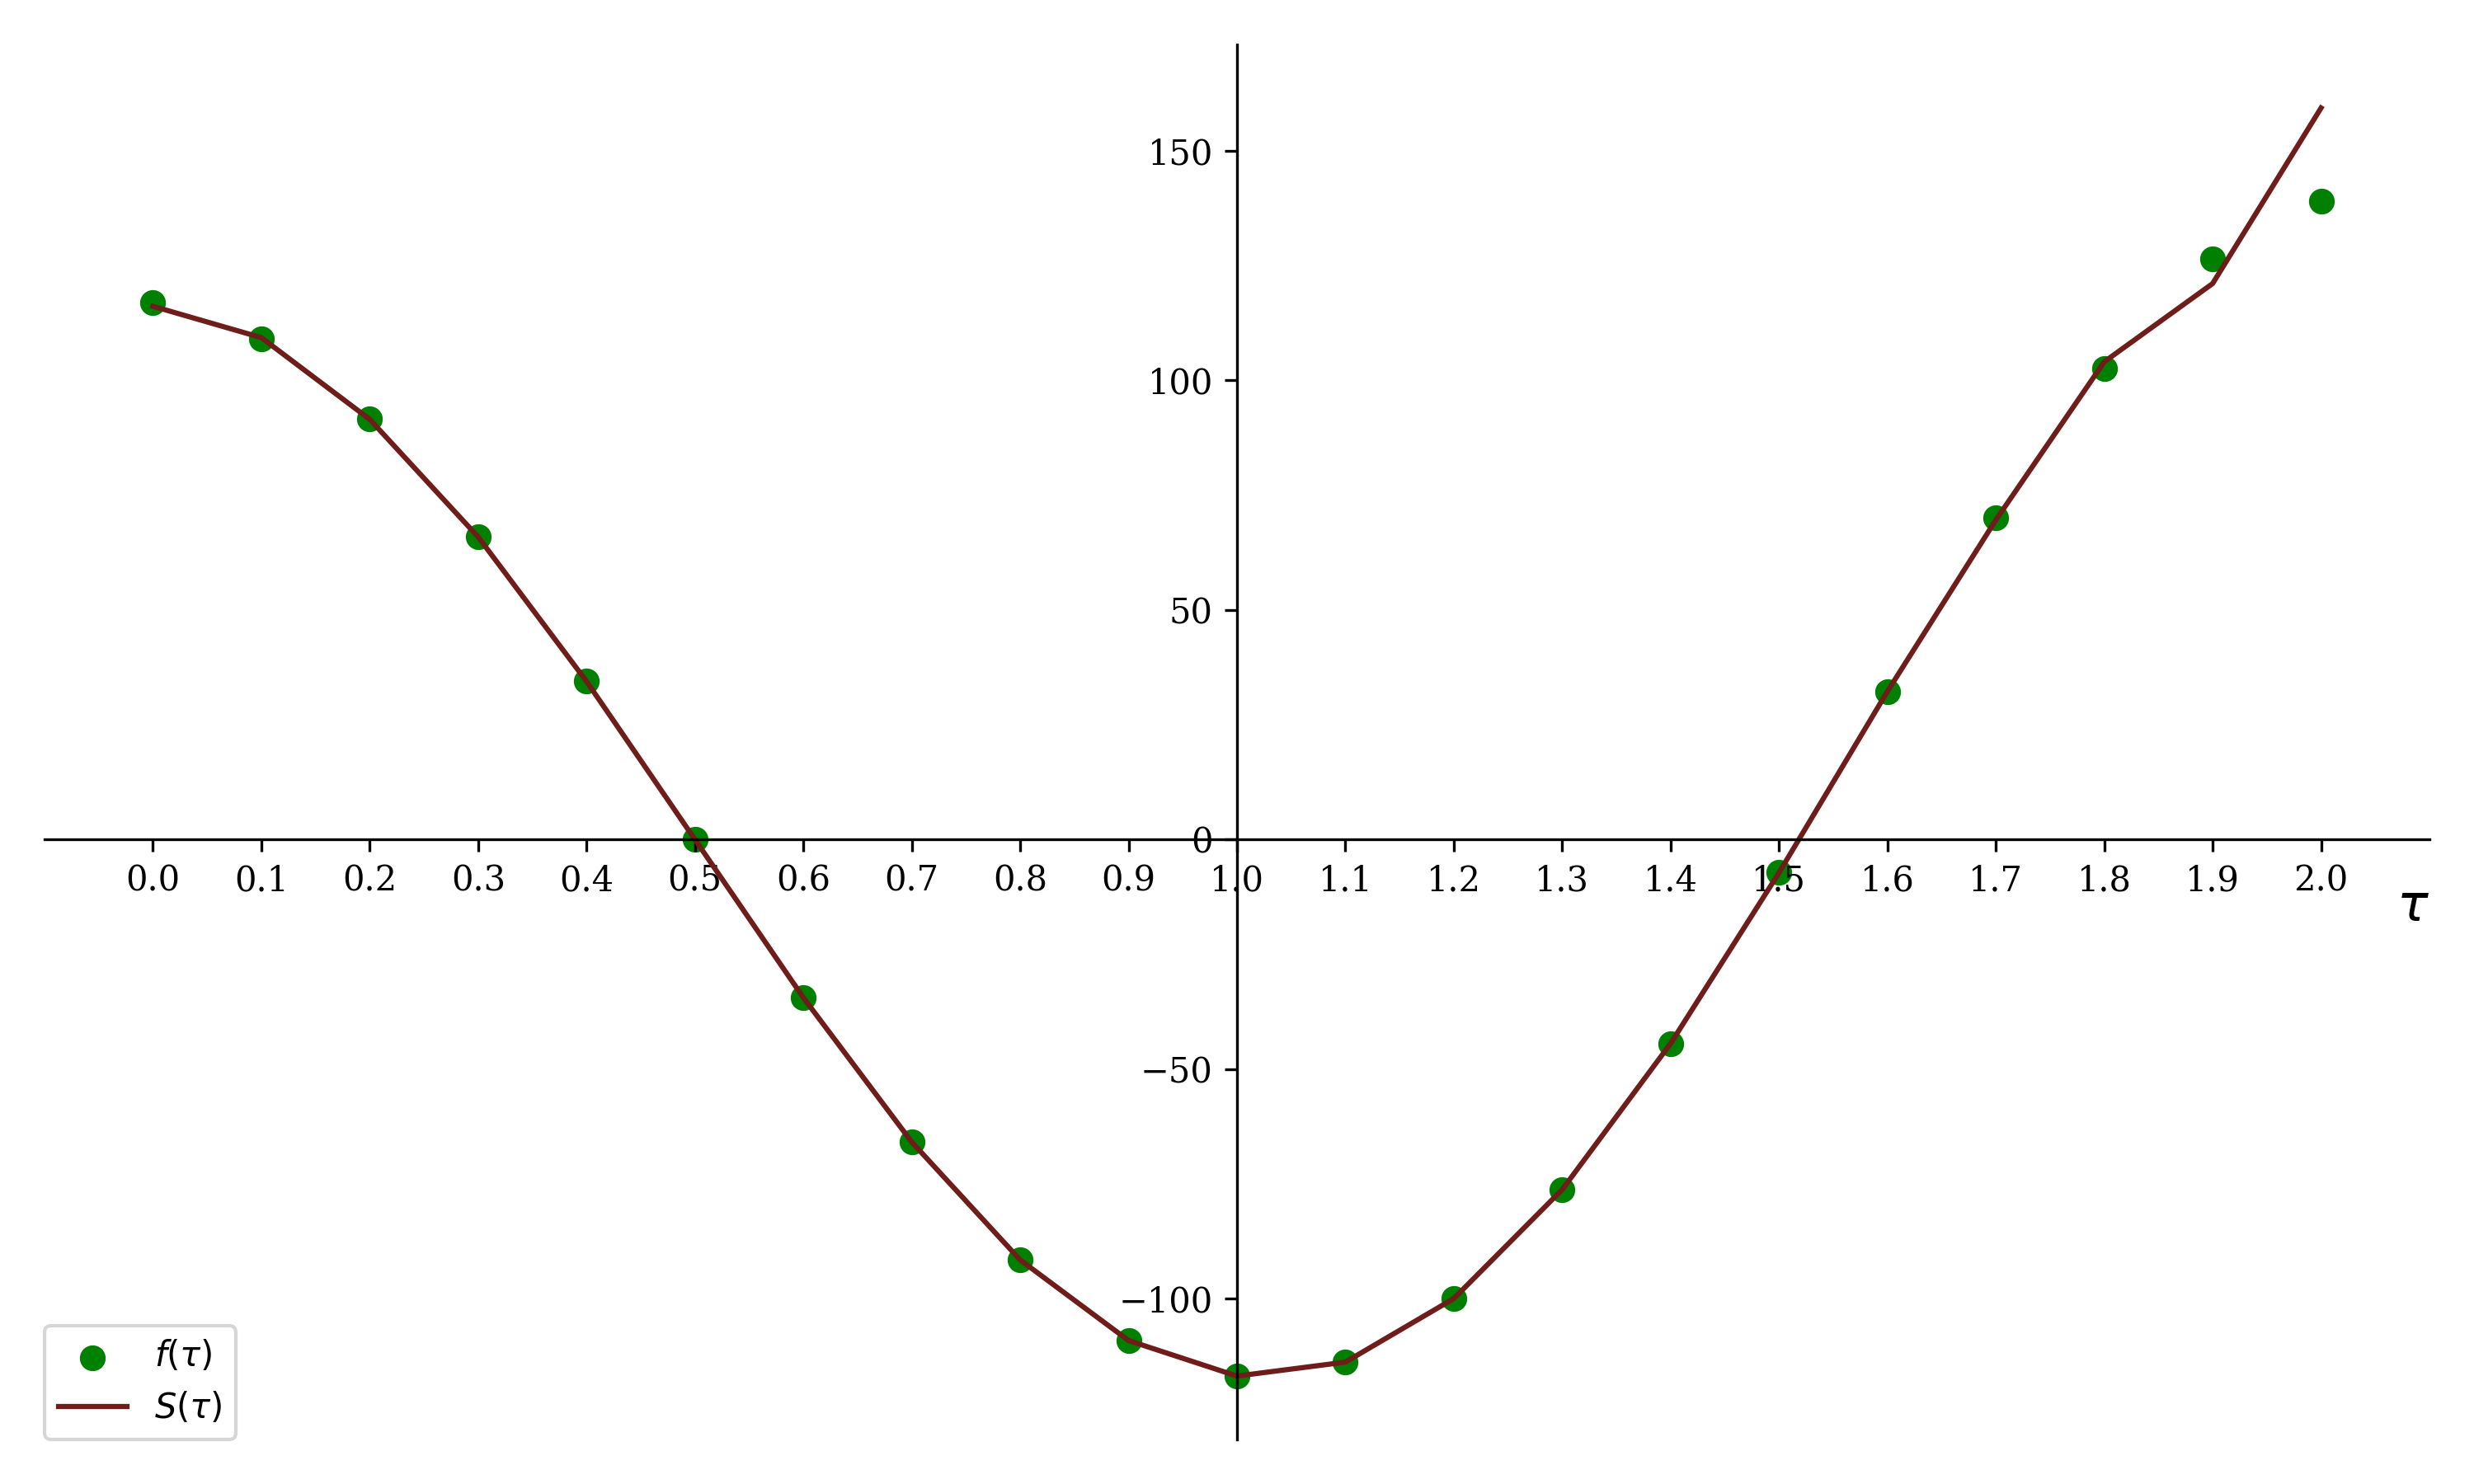
\includegraphics[width=1\textwidth]{mainDiff_x_splineDiff_20}
\end{center}

\vfill

\newpage

k = 40:

\begin{gather*}
    f'(\tau) = \langle 116.874, 114.31549, 109.14201, 101.49801, \dots, 134.38322, 139.08424 \rangle \\
    S'(\tau) = \langle 116.52112, 114.40966, 109.11642, 101.50455, \dots, 132.55742, 145.89636 \rangle 
\end{gather*}
 
\begin{center}
    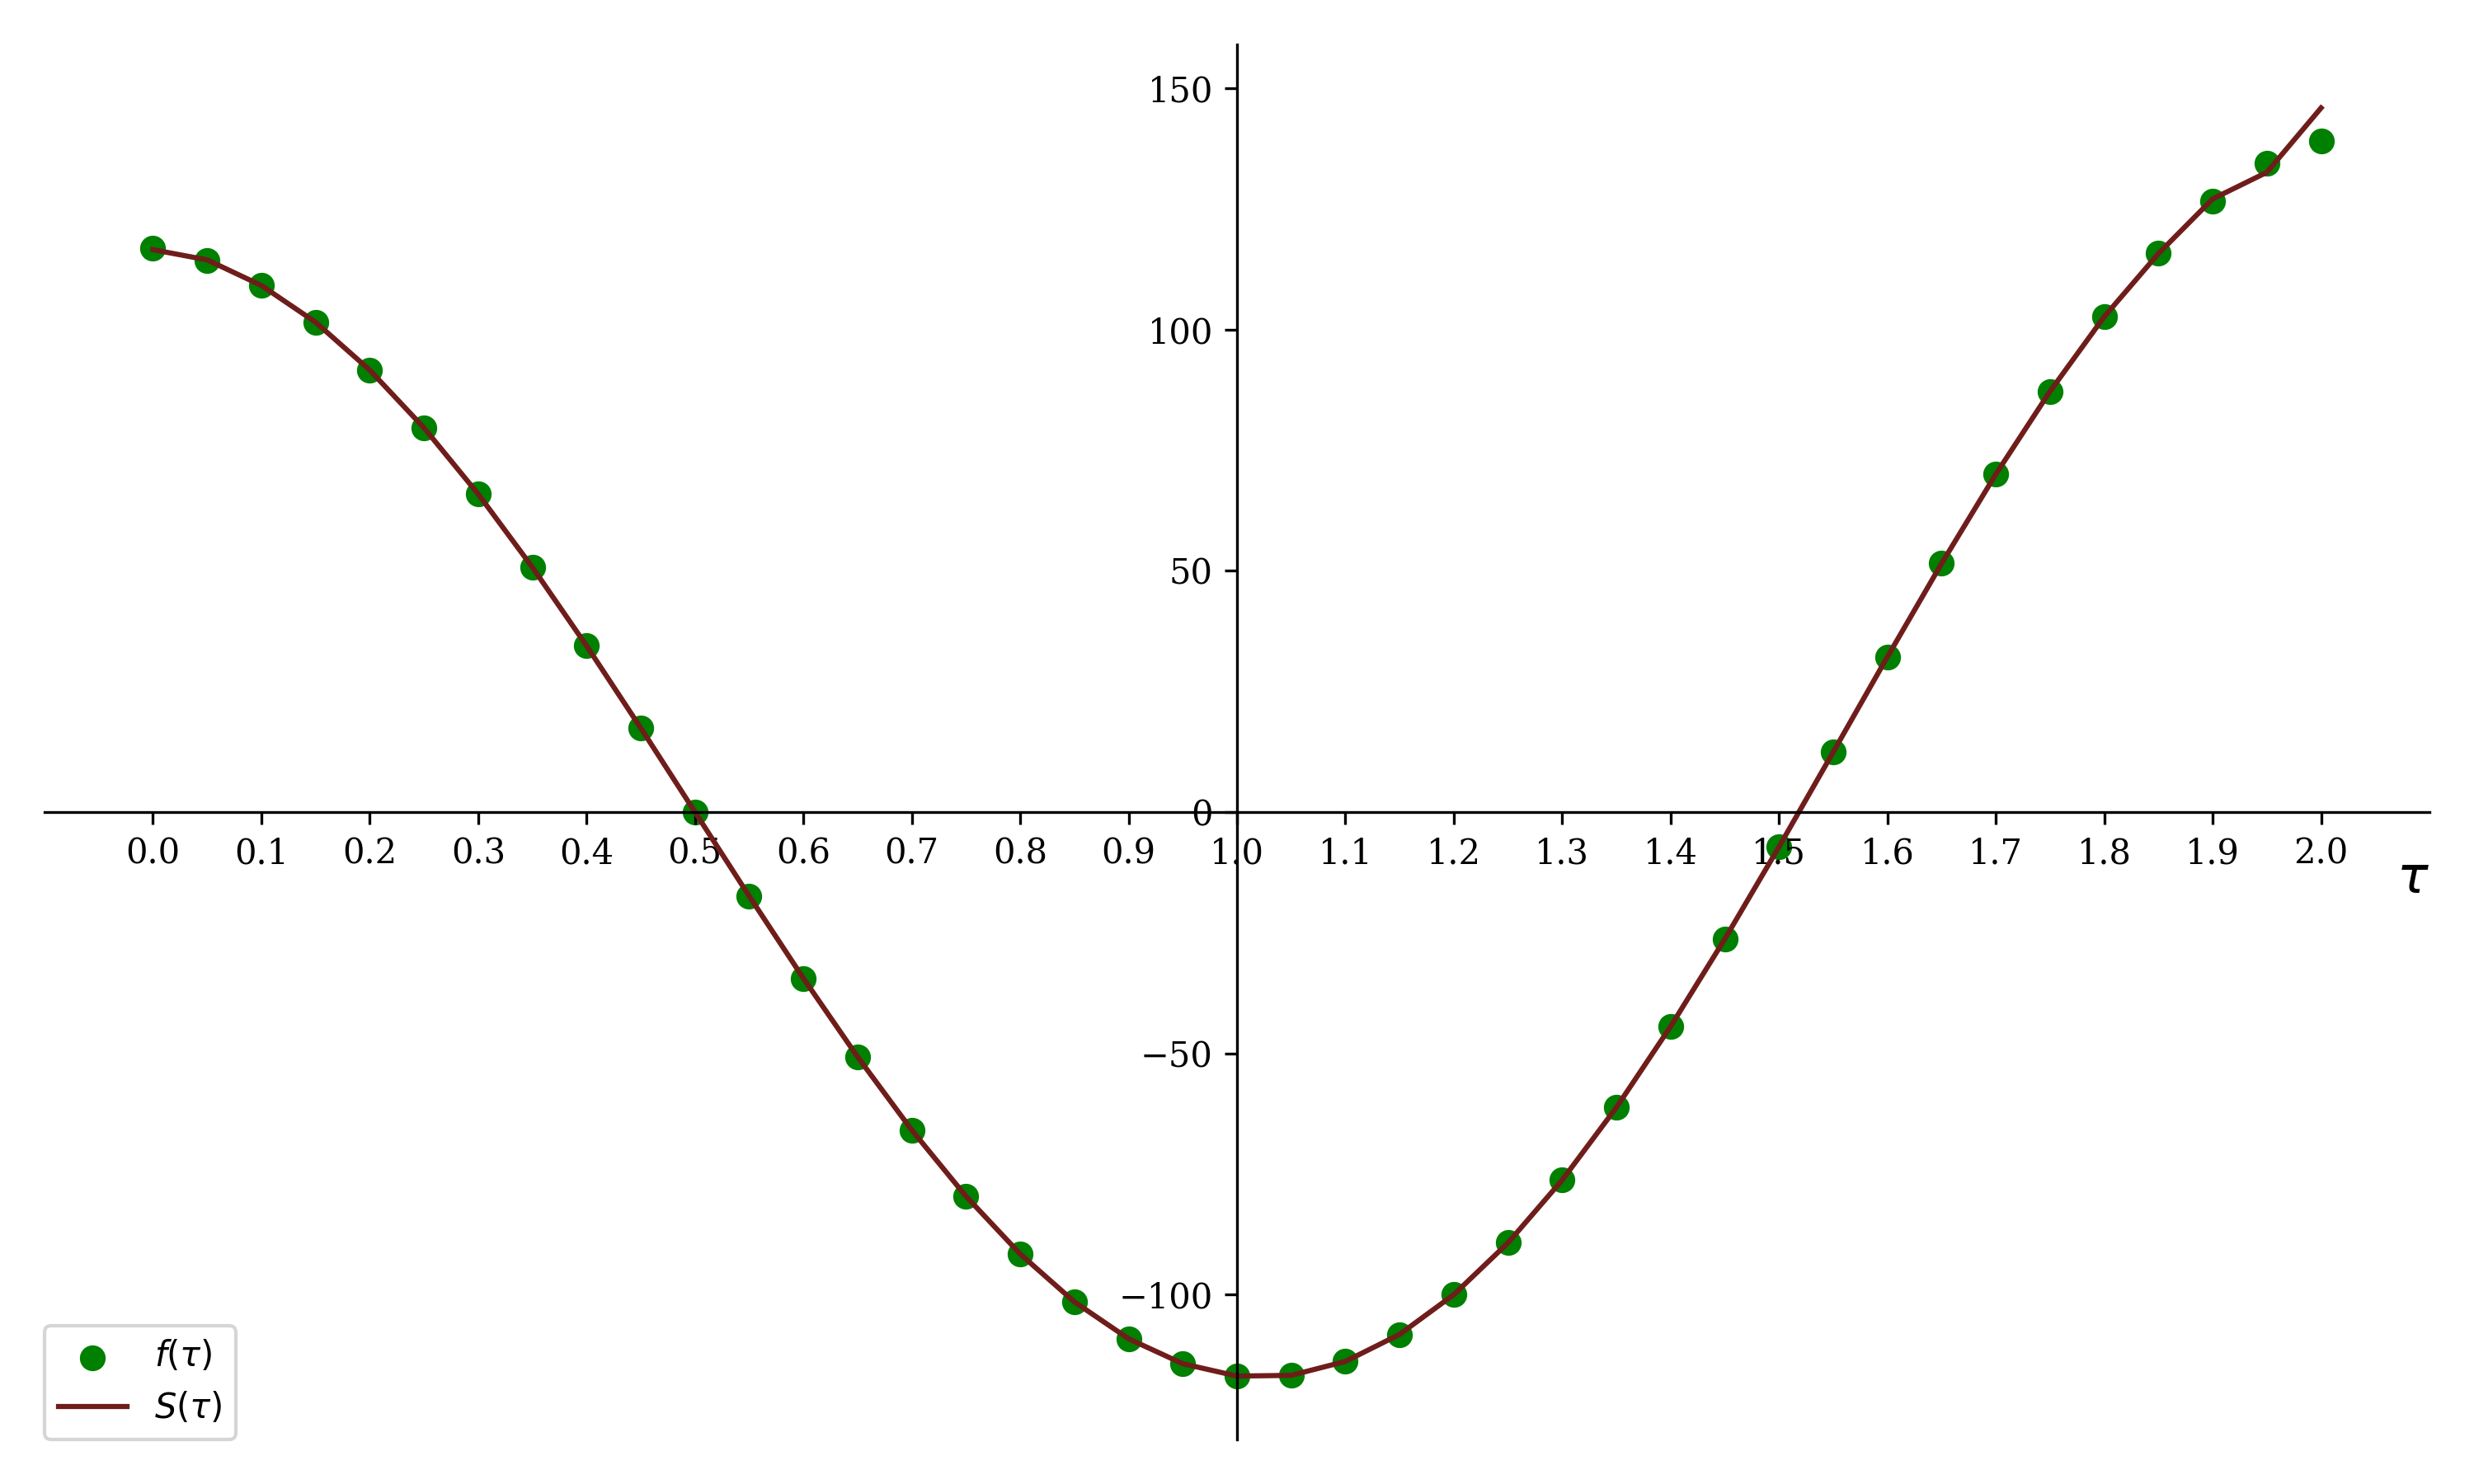
\includegraphics[width=0.85\textwidth]{mainDiff_x_splineDiff_40}
\end{center}

k = 100:

\begin{gather*}
    f'(\tau) = \langle 116.874, 116.17146, 115.0401, 113.48611, \dots, 137.59343, 139.08424 \rangle \\
    S'(\tau) = \langle 116.73348, 116.2091, 115.03, 113.48881, \dots, 137.08692, 140.9745\rangle 
\end{gather*}
 
\begin{center}
    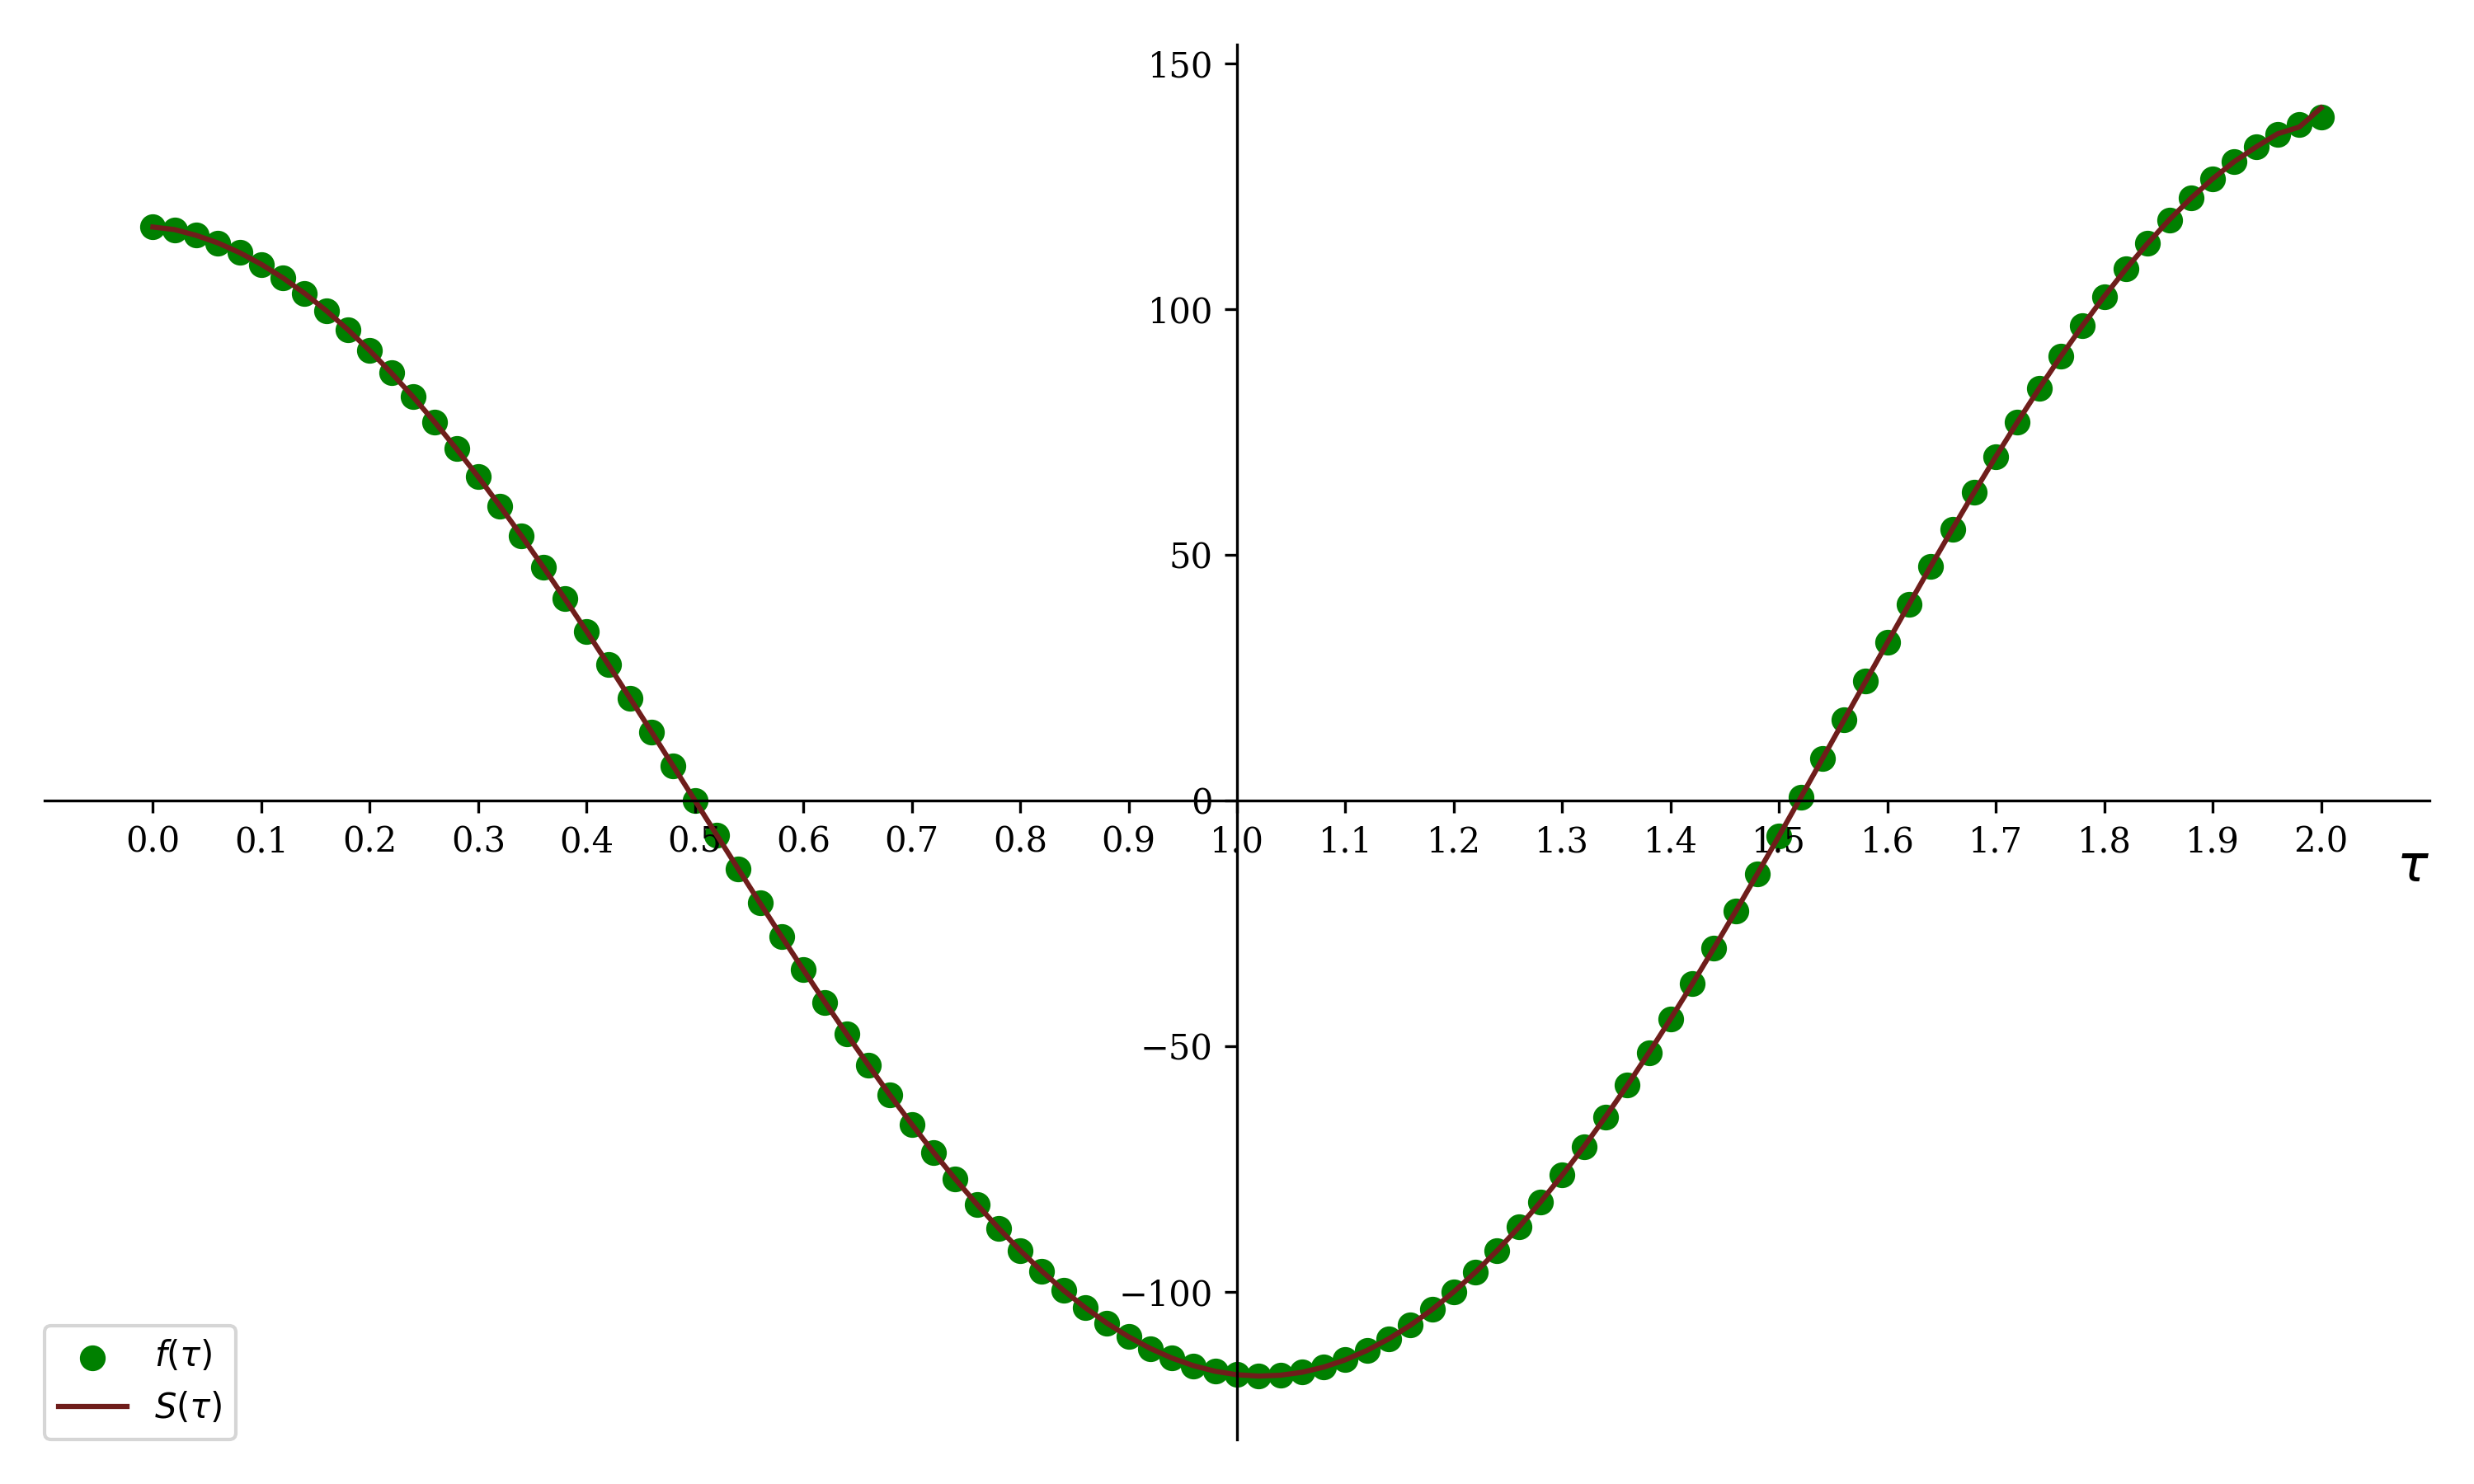
\includegraphics[width=0.85\textwidth]{mainDiff_x_splineDiff_100}
\end{center}

\end{document}
